\documentclass{article}

\usepackage{enumitem}
\usepackage[a4paper, margin=0.8in]{geometry}
\usepackage{graphicx}
\usepackage[hidelinks]{hyperref}
\usepackage[os=mac, mackeys=symbols]{menukeys}
\usepackage{titlesec}
\usepackage{xcolor}

% Roll credits...
\title{Avara Documentation}
\author{Jack “Orvis” Lawrence and “Cajun” David Richard}
\makeatletter
\hypersetup{
    pdftitle = {\@title},
    pdfauthor = {\@author}
}
\makeatother

% Section formatting
\titleformat*{\section}{\huge\sffamily}
\titleformat*{\subsection}{\large\bfseries\color{blue}}
\titleformat*{\subsubsection}{\bfseries}
\titlespacing{\section}{0pt}{\parskip}{-\parskip}
\titlespacing{\subsection}{0pt}{\parskip}{-0.25em}
\titlespacing{\subsubsection}{0pt}{\parskip}{-0.5em}
\let\oldsection\section
\renewcommand\section{\clearpage\oldsection}

% Set document fonts
\renewcommand{\rmdefault}{ptm}	% Times
\renewcommand{\sfdefault}{phv}	% Helvetica
\renewcommand{\ttdefault}{pcr}	% Courier

% TOC stuff
\setcounter{tocdepth}{2}	% Show subsections
\renewcommand*\contentsname{2\hspace{0.5cm} Table of Contents\\*[-0.5em]\rule{5.5cm}{.15pt}}
\newcommand\invisiblesection[1]{
	\refstepcounter{section}
	\addcontentsline{toc}{section}{\protect\numberline{\thesection}#1}
	\sectionmark{#1}
}

% Paragraph formatting
\setlength{\parindent}{0em}
\setlength{\parskip}{.8em}
\setlist{nosep}

\begin{document}
\invisiblesection{Welcome to Avara}

\begin{center}
	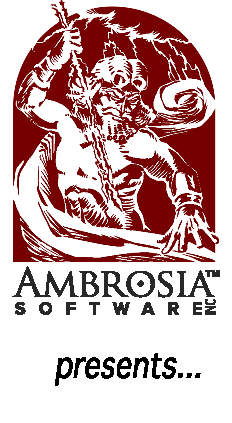
\includegraphics[width=1.542in]{img/01.pdf}\\
	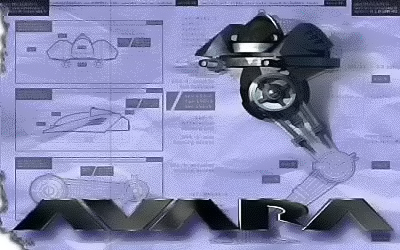
\includegraphics{img/02.png}
\end{center}
\rule{5.5cm}{0.15pt}\\
\textbf{Documentation} \textit{by Jack ``Orvis'' Lawrence and ``Cajun'' David Richard\\
Special thanks to Andrew Welch and Ms. Howard\\
©1996 by Ambrosia Software}

\subsection{Welcome to Avara}
Once again, Berserkir sat, licking his wounds and nursing his pride. An unsavory defeat against his nemesis, Achilles, had left a bitter taste in the haughty warrior's mouth. Under a furrowed brow however, Berserkir's thoughts dwelt upon revenge, not defeat.

Time would pass and again, at Mount Stonehammer they met. Two warriors, side by side, walking with the purposeful countenance that only the spectre of death could imbue. The trees were still. The birds were quiet. Even Father Wind held his breath in silent anticipation of the struggle that would shake the very mountaintops. Focusing on all the training he had endured and with strong will and determination, he conquered the mighty Achilles. Father Wind breathed a sigh of relief as the battle ended, carrying the soul of Achilles on the heels of his autumn breeze.

Are you prepared for battle? Are you ready for Avara? With its fast and furious action and unique 3D game play, you can't help but be absorbed in the game. Avara's real-time graphic action will start your heart pounding as you see your opponent gracefully bound across the terrain and quickly swoop in behind you. Using both the mouse and keyboard, you have complete 360 degree control to counter-maneuver and quickly target your enemy. Players aren't limited to ``sliding'' around in predetermined mazes like in many of the older 3D games. Avara's maneuverability is unique, allowing its warriors to freely climb, jump, and run on any of the structures in the battlefield.

Add to this Avara's networkablity, and the game gets even more interesting. Avara allows you to meet and play against people from all around the world, right over the Internet. Develop your skills and strategy in the many solo levels, and when you are ready, access the Avara Internet Tracker to locate worthy opponents. The Tracker offers users a continually updated list of Avara games in progress all over the net. Avara can also be played across LAN (Local Area Network) connections, for those not brave enough to step out into the maelstrom of Internet battle.

With Avara, you are also able to design your own battlefields. The only limiting factor to your gaming experience is your imagination. Using the objects and structures that are provided, and an easy-to-follow manual, designing levels for Avara is a snap. You will never get tired of Avara due to this expandability; it is a game that is always growing. New and exciting levels, from those who want to show off their creative and imaginative accomplishments, will spread all over the Internet.

\subsection{About This Manual}

This manual assumes that you are familiar with the Macintosh and its basic operation. If you need help using the mouse, choosing from menus, or working in the Finder, please consult the \textit{Macintosh User's Guide} that came with your Macintosh, or the online \textbf{Apple Guide} from the \textbf{Balloon Help} menu.

\subsubsection{If you don't like to read manuals\dots}
Go directly to Chapter 4, \textit{Getting Started}. This chapter briefly describes how to get Avara up and running in just a few minutes. The details of the game are described in the remainder of the documentation.

\subsubsection{If you prefer step-by-step instructions\dots}
Chapter 4, \textit{Getting Started}, has many useful tips that will help you when playing Avara. You should read it and then continue on to Chapters 5 through 12, which explain the game in more detail. They provide all the specifics of the game that can not be learned through playing.

Chapter 13, \textit{Avara Extras} describes some of the extra items that come with Avara, such as the \textit{Avara MicroTracker} and \textit{Avara Commuter}, and gives information about building and editing your own levels.

Chapter 14, \textit{Optimization and Troubleshooting}, and Chapter 15, \textit{Menu Descriptions}, are reference chapters. The \textit{Optimization and Troubleshooting} chapter discusses how to get the best performance from your Macintosh and your network, and also answers some common questions that arise. The \textit{Menu Descriptions} chapter details the operation of each menu item in Avara.

\subsubsection{To use this manual as a reference\dots}
See Chapter 2, \emph{Table of Contents}, for an outline of this manual. Under each heading is a listing of the points covered in that chapter.

% TOC
{\setlength{\parskip}{0.1em}
	\invisiblesection{Table of Contents}
	\tableofcontents
}

\section{About Avara}
\rule{5.5cm}{.15pt}\\
\rmfamily\textit{An introduction to the wide open spaces}

\begin{center}
	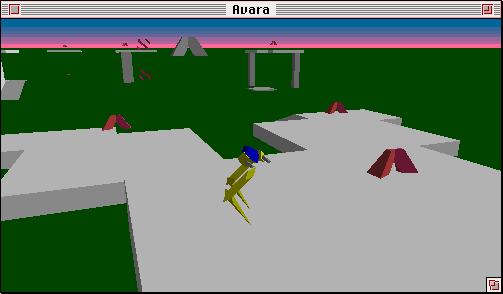
\includegraphics[width=\textwidth]{img/03.png}
\end{center}

\subsection{A True 3D World}
Avara is a true 3D environment. Unlike other ``3D'' games, Avara allows for the third dimension to be fully realized. In the world of Avara you are able to climb stairs, jump, walk along the top of platforms or walls, or through buildings. You can navigate labyrinthine corridors, or dark landscapes. This environment offers infinite possibilities for level designers and players alike.

Your vehicle in the world of Avara is the \textbf{H}ostile \textbf{E}nvironment \textbf{C}ombat and \textbf{T}ransport \textbf{O}perations \textbf{R}emote unit, affectionately known as the \textbf{H.E.C.T.O.R.} The HECTOR is controlled with the keyboard and the mouse. Keyboard commands allow the HECTOR to walk forward or, backward, to turn, to crouch, to jump, and to use a variety of weapons. The head, or ``pod'', of the HECTOR is controlled with the mouse. Its movement is completely independent of the body and can sweep in an arc of approximately 100 degrees left and right of center, and vertically approximately 60 degrees both up and down.

For more information, see Chapter 7, \textit{The H.E.C.T.O.R.}

\subsection{Challenging Solo Levels}
Sure, the HECTOR is the baddest combat vehicle around, but Avara is more than just blasters and missiles. Because of the rich nature of the game, Avara sometimes presents situations where alternative solutions must be found. In the many solo missions, the problem isn't always solved with grenades. You will need agility and cunning as well.

Each solo missions presents you with a goal to reach. This goal is in the form of a transporter marked with a star. You need to reach this transporter so that you can continue on to the next mission. This is done by manipulating the objects in the mission and opening new pathways for your HECTOR to traverse. Oh yes, you might also have to duke it out with the various enemies on each level.

When playing the solo levels, explore the structures and try different approaches. Sometimes there is more than one way to solve the puzzle.

\subsection{Competing with Others}
Avara also offers the ability to use a networked Macintosh to play against others. Many network levels provide arenas for players to test their cooperative skills, or to fight to the death against each other. Network Avara can be played locally with an AppleTalk network, or over the Internet.

Avara is equipped with network-savvy features. While connected to the Internet, you can easily check to see if other players are on the Internet looking for a game. You can also offer an invitation for others to join your game by registering it with the Avara Tracker. The Avara Tracker is a program that is always running on the Internet server in the Ambrosia home office. It makes finding opponents on the Internet simple, and fast.

Avara has an Internet chat capability that makes communicating with the other players in your game convenient. Avara also indicates where the players are located on the globe. You can even see what your opponent looks like! Player can paste pictures of themselves (or of anything else) into their copy of Avara so that others can see who they are.

\subsection{Keeping Up with the Ever-Changing World of Avara}
Ambrosia is sponsoring an Avara web site at \textbf{\href{https://web.archive.org/web/20000302231943/http://www.avara.com:80/}{\texttt{http://www.Avara.com}}} where you can find all the latest and greatest news about Avara. The Avara HyperArchive has loads of information designed to help you get the most out of Avara. Avara.com is where the Avara Tracker resides. There is also a Mission Exchange forum where you can download all the best new missions, or upload your own creations! Drop by to see what's up with Avara!

Although Ambrosia sponsors Avara.com, they don't maintain it and are not responsible for its content. For more information on getting in touch with Avara.com, stop by the web site.

\subsection{System Requirements}
\begin{itemize}
	\item Color Capable Macintosh
	\item System 7 or later
	\item 4000K of free RAM
	\item 10MB of hard drive space
	\item Network connection for local network play
	\item Direct Internet connection for Internet play
\end{itemize}


\section{Getting Started}
\rule{5.5cm}{.15pt}\\
\rmfamily\textit{A quick start guide to Avara}

When you first launch Avara, you are shown several windows. Each window contains controls and information for the different aspects of the game. The windows are explained in greater detail later in the documentation, but for now we will concentrate on getting a Player File set up, learning the keys used to pilot a HECTOR, loading a mission, and starting and pausing the game. Most important, this chapter explains why you should save your game right away.

\subsection{Saving Your Game}
This first thing you should do when you open Avara for the first time is type your name in the ``Player Name'' field. The ``Player Name'' field is in the Player window, and should be the upper-left most window on your screen. After you type your name in the Player window, choose Save As\dots\ from the File menu and save the game in the Avara folder (or wherever you like).

\begin{center}
	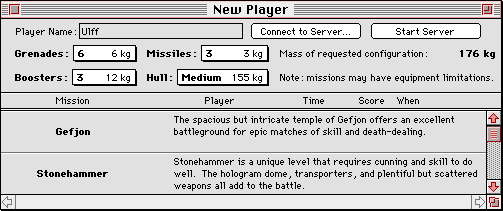
\includegraphics[width=\textwidth]{img/04.png}
\end{center}

Avara will save your game as you play, but first you need to create a file so that Avara knows where to save your data. This file will be automatically updated as you play.

\subsection{Piloting a HECTOR}
The next thing you need to know are the basic controls used to pilot a HECTOR. The HECTOR is the vehicle you use to interact with the world of Avara.

Choose \textbf{Keyboard} from the \textbf{Window} menu. This brings up the Keyboard Editor window. In this window, you will see a keyboard map and a listing of controls with associated icons. The Keyboard Editor window has a drag and drop interface. You can click on the various icons in the window to see which controls they represent and what they do. To assign a control to a key, simply drag the icon onto the desired key in the keyboard map. To remove a control from the keyboard, drag the icon off the key and back into the icon field.

\begin{center}
	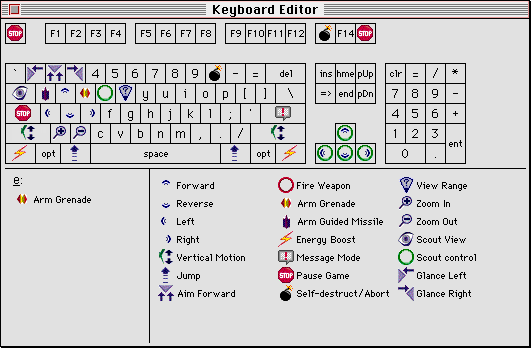
\includegraphics[width=\textwidth]{img/05.png}
\end{center}

You can assign multiple controls to one key. The default keyboard layout has an example of this. The \textbf{\keys{C}} key is set to both load, and fire a grenade. It is a quick way to get off a shot.

In all cases, your mouse will control the head of the HECTOR. Your mouse button will always fire the currently selected weapon. All other controls are on the keyboard. This includes all other movements of the HECTOR.

If you like to learn a game by playing it, try leaving the Keyboard Editor window up while you play so that you can pause the game and refer to the key mapping.

\subsection{Loading a Mission}
Avara missions that are available to play are listed in the lower portion of the Player window. This is the window where you typed your name. The first (and at this point, only) mission available is called Training Course. Click once anywhere in the rectangle where Training Course is listed. Avara will load this mission. As you complete missions, other missions become available to you. To load any listed mission for play, just click on the mission.

\subsection{Pausing and Starting a Game}
After you have a Mission loaded, the next thing you need to know is how to pause the game.

``PAUSE the game? But I haven't even STARTED yet!''

When you play Avara, the mouse is used to control the HECTOR. That means that while Avara is running, there is no cursor and you won't have access to any of the menus or controls on your Macintosh. To get your cursor back, you need to pause the game.

By default, both the \textbf{\keys{Esc}} key and the \textbf{\keys{Delete}} key will pause Avara. You can use the Keyboard Editor window to change these keys or set new ones according to your preference.

Now to the good part, STARTING the game.

You can start an Avara mission by choosing \textbf{Start} from the \textbf{Game} menu, or by pressing \textbf{\keys{\cmd-R}}. When you do this, the Game window will come forward and the mission will start.

If you have paused Avara, you can continue the mission by choosing \textbf{Resume} from the \textbf{Game} menu, or by pressing \textbf{\keys{\cmd-R}}.

\subsection{Loading in a Different Set of Missions}
In order to display a new set of missions in the Player window, choose \textbf{Open\dots} from the \textbf{File} menu and select any set of Avara missions on your Macintosh. When you have opened a new set of missions, you will see the missions listed in the Player window change. To load a mission from the new list, just click on it.


\section{Elements of Avara}
\rule{5.5cm}{.15pt}\\
\rmfamily\textit{Looking through the windows}

Avara has several windows: some are used during game play, and others are used to configure and set up games. The windows are the \textbf{Keyboard Editor Window}, the \textbf{Player Window}, the \textbf{Roster Window}, the \textbf{Instruments Window}, and the \textbf{Game Window}. Each one is described below:

\subsection{Keyboard Editor Window}
\color{black}
\begin{center}
	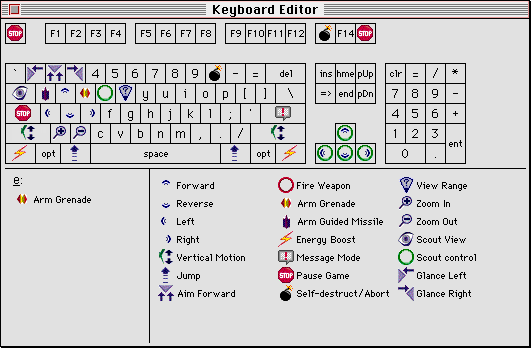
\includegraphics[width=\textwidth]{img/05.png}
\end{center}

The Keyboard Editor window is used to set the keyboard controls of the game. The top half of the window displays a keyboard map depicting the keyboard you have connected to your computer. In the lower right portion of the window are listed all the controls for the game along with their identifying icons. Each control or key is described in the lower left portion of the window. When a key is set to a particular control, the icon for that control is displayed on the keyboard map.

\subsubsection{Getting the Description of a Key or Control}
The description area gives you important information about the various controls of Avara. When you click on one of the control icons, you will see the name and description of that control in the description area. Clicking on a key in the keyboard map with your mouse will display the key and the associated control in the description area. If you strike a particular key on your keyboard, the description area will show you what control or controls are assigned to that key.

\subsubsection{Changing Settings}
Changing the settings for the keyboard is as easy as dragging and dropping. To assign a control to a key, simply drag the icon for that control from the lower right area and drop it on the desired key in the keyboard map. To remove a control from a key, drag the icon off of the key in the keyboard map and drop it into the lower right area of the window.

There is another way to do this. Click on one of the keys in the keyboard map, and the description area will indicate the key you selected. You can then set the control by dragging the icon into the description area.

You can assign the same control to multiple keys by dragging the control icon to all the keys you want to associate with that control.

\subsubsection{Combining Actions}
Avara lets you assign multiple controls to a particular key. Suppose you would like the ability to load and launch a grenade in one step. Select the key that you would like to set, and drag the icons for ``Load Grenade'' and then ``Fire Weapon'' onto the key. Order is not important. You could accomplish the same thing by dragging multiple icons into the description area after selecting a key. When you use this key during play, a grenade will be loaded and launched with one keystroke.

\subsubsection{Saving a Keyboard Layout}
It is a good idea to save your keyboard setup. In order to do this, you must be working in the Keyboard Editor window. Choose Save\dots\ from the File menu and name your keyboard settings whatever you like.

\subsection{Player Window}
\begin{center}
	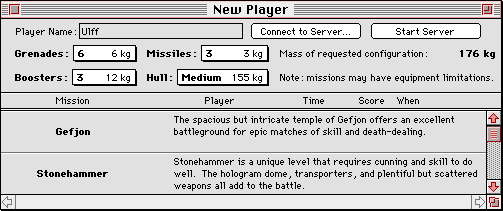
\includegraphics[width=\textwidth]{img/04.png}
\end{center}

The Player window has several elements:

\subsubsection{Player Name}
This is where you should type the name you will play under, your ``Avara handle.'' This is how people playing with you know who you are. When you first start Avara, the ``Player Name'' field is highlighted. Type in your name and select \textbf{Save\dots} from the \textbf{File} menu to save your Player file. After you save your game, Avara will remember your name and display it as the title of the Player window.

\subsubsection{Connect to Server/Start Server buttons}
These buttons are used to play Avara as a network game. For more information on playing network Avara, see Chapter 9, \textit{Network Avara}.

\subsubsection{Hull and Weapon Pop-up Menus}
You can use these menus to set the hull type and the weapon carrying capacity of your HECTOR. The total weight of the configuration you have selected is displayed to the right of the pop-up menus. Lighter hulls have a lower maximum weapon capacity, so some selections on the menu may be gray to indicate that they are not available for the hull you have selected. If you want to carry more weapons, you need to first select a heavier hull. Be careful though: the heavier you are, the more slowly you will move. For more information on your HECTOR and its weapons, see Chapter 7, \textit{The H.E.C.T.O.R.}

\subsubsection{Missions}
The missions that are available for you to play are listed in the lower portion of the Player window. The list of available missions may be longer than can be displayed in the Player window. If this is the case, you can use the scroll bar to the right to see additional missions.

Avara comes with a series of missions built in. Successfully completing a mission makes more missions available to play. To display another set of missions in the Player window, select \textbf{Open\dots} from the \textbf{File} menu and browse through the folders or drives on your Macintosh to find other sets of missions.

If you wish to play the original missions again, select \textbf{Use Built-In Missions} from the \textbf{Game} menu.

Avara allows players to create new missions or edit existing ones. See Chapter 13, \textit{Avara Extras} for more information on making your own levels.

If you have not played a particular mission before, a brief description of that mission is shown next to its name. When you play a mission, information about how well you did is saved to your Player file and displayed in the mission section of the Player window. Each time you play a mission, this information is updated.

If you do not want Avara to update your Player file automatically, you need to deselect \textbf{Save Results Automatically} from the \textbf{Game} menu.

To see the description of a mission you have already played, move your cursor to that field and hold down the mouse button. Releasing the button will load the mission. If you do not want to load the mission, move your cursor out of the Player window.

\subsubsection{Loading and Playing a Mission}
To load a mission, simply click anywhere in the field that describes the mission. After the mission loads (it may take a second or two), information about the mission is displayed in the lower portion of the Roster window. If you want to play a different mission, just click on a new one in the Player window.

You can begin the mission by selecting \textbf{Start} from the \textbf{Game} menu, or by pressing \textbf{\keys{\cmd-R}}. The Game window will come forward and the mission will start.

When Avara is running a mission, the mouse is used for operating the HECTOR. If you need to get your Macintosh cursor back or you want to pause the mission, you need to hit the ``Pause'' key (\textbf{\keys{Esc}} or \textbf{\keys{Delete}} by default). When your mission is paused, the cursor comes back allowing you access to the menus and windows of Avara or of any other program. You can load a different mission if you like, or a new set of missions, or you can continue the current mission by selecting \textbf{Resume} from the \textbf{Game} menu, or by pressing \textbf{\keys{\cmd-R}}.

\subsection{Roster Window}
The Roster window is a storehouse of information about the game in progress. It displays your status, the status of any other players in the game, information about the mission that is currently loaded, communications between you and the other players, and the results of any mission you play.

The lower portion of the Roster window shows additional information about the level that is currently loaded, included the amount of time given to complete the mission.

Much of the information in the Roster window pertains to network games of Avara. For more information on playing Avara as a network game, see Chapter 9, \textit{Network Avara}.

\subsubsection{The Tabs}
The Roster window has a number of tabs along the bottom that can be selected to display various information about Avara. To see what is on any particular tab, just click on it with the mouse. Each tab is discussed below.

\begin{center}
	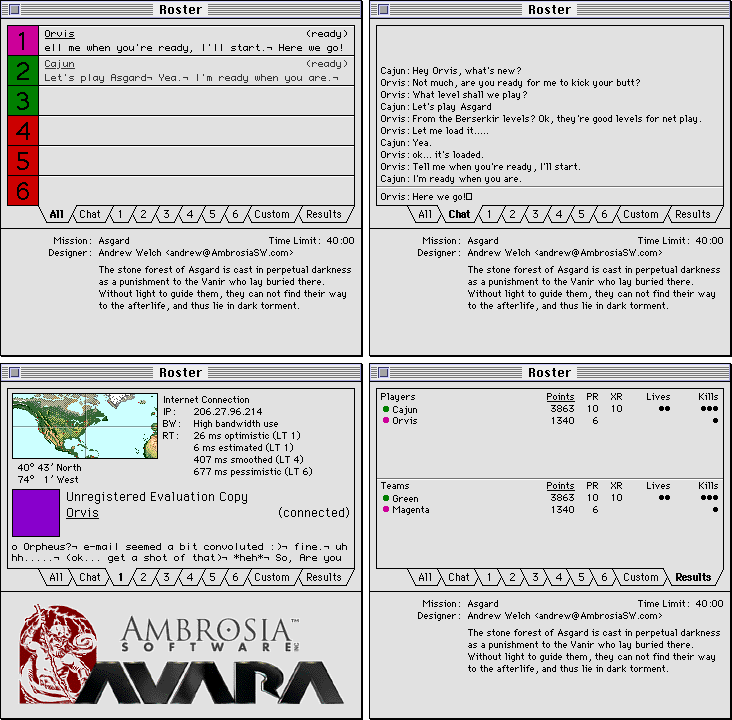
\includegraphics[width=\textwidth]{img/06a.png}\\
	\sffamily{\footnotesize\textbf{The Roster Window:} Four different views}
\end{center}

\subsubsection{All}
The ``All'' tab shows a list of all the players in a game as well as their status and their individual or team colors. To change the color of your HECTOR, click on the color box to the left of your name. A pop-up menu appears, and you can select a new color. You cannot change the color of your HECTOR in a mission that has already started.

If you are playing Avara as a network game, you will see all of the players' names on this tab. Avara can accommodate up to six players in a network game.

A player's status in the game is displayed to the right of his or her name. A (ready) status indicates that a mission is ready to be started. An (active) status is displayed when a mission is running. If a player pauses a mission, the status area shows (paused). Many different status messages can be displayed. Most of them apply to Avara as a network game.

The lower portion of each player field is used to display any text that players type to each other between or during the missions they play.

\subsubsection{Chat}
The ``Chat'' tab presents an IRC-style chat window. Players in a network game of Avara can send messages to each other by typing, and all the text is sent to this window. The text sent by individual players is also displayed in other windows and tabs. For instructions on how to use the chat feature of Avara, see Chapter 9, \textit{Network Avara}.

\subsubsection{The Player Tabs}
Tabs ``1'' through ``6'' display information about each player in the game. In the upper left corner of this tab is a map that displays your geographical location. Avara reads this information from the \textbf{Map} control panel of your Macintosh. To set this information, open the Map control panel, enter your latitude and longitude in the proper boxes, and click on the ``set'' button. You can also click on the map to select a specific location.

To the right of the map is an area that allows you to insert a picture of yourself (or of anything else). If you have a picture in this location, other players in a network game will see it. It's a great way to personalize your copy of Avara!

Avara allows you to paste in an image of up to 64$\times$64 pixels. There are many programs available that will allow you to create such an image, but their use is beyond the scope of this manual. Some sample images are included in the Avara distribution to help get you started.

To put an image into the Roster window, you first need to open the image with any image editing program. If you are not sure how to do this, try double-clicking on the image. Once it is open, select the image and then choose \textbf{Copy} from the \textbf{Edit} menu. Now, select your tab in the Roster window and choose \textbf{Paste} from the \textbf{Edit} menu. Your picture should now be in the window! Avara will automatically save this information, and your picture should appear in the same place the next time you run Avara.

Below the map is a square that represents the color of your HECTOR. You can change your color here the same way you did on the ``All'' tab. Simply click on the square and a menu of colors will pop-up. Select any color you wish.

Your Player Status from the ``All'' tab is also displayed here, as is your Player Name and whether or not have you are using a registered version of Avara. All the players in a network game can see the information on your tab, and you can see theirs by selecting their tabs.

At the bottom of a Player tab is another field that displays only the chat-text that you type. Each player's tab will display the chat-text they have typed.

There is more information displayed on this tab in a network game of Avara. For more information, see ``The Roster Window Revisited'' in Chapter 9, \textit{Network Avara}.

\subsubsection{Custom}
The ``Custom'' tab is used to display information from customized Avara plug-ins. A plug-in might be used to tabulate scores. For more information on plug-ins, see Chapter 13, \textit{Avara Extras}.

\subsubsection{Results}
The ``Results'' tab displays individual and team scores for an Avara mission.

\subsection{Instruments Window}
\begin{center}
	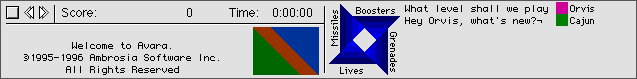
\includegraphics[width=\textwidth]{img/07.png}
\end{center}

In the Instruments window you will find all of the information that is important to you during a mission. Your score, time, weapons, shield status and other information can be found here. Many monitors are not large enough to display all the windows of Avara with no overlap, but you will want to make sure that you can see your Instruments window while you are playing.

The layout of the Instruments window can be changed to suit your monitor and your preference. By clicking on either of the opposing arrows at the top-left of the window, you can cycle through four different layouts. Some layouts will conserve space by not displaying the console or communications portion of the window. Each of the four layouts will show your score, lives, time, and the status of your energy, shields, and weapons.

\subsubsection{Elements of the Instruments Window}
There are several elements in the Instruments window. They are broken down into five fields: \textbf{Power}, \textbf{Weapons/Lives}, \textbf{Console}, \textbf{Communications} and \textbf{Score/Time}. Some configurations of the Instruments window do not display every field.

\textbf{Power}: Your power is displayed as a three-part graphic. This graphic is rectangular with a brown stripe laid diagonally across it. This creates two triangles. The left triangle is green and represents your energy. The right triangle is blue and represents the strength of your shields. The brown stripe is actually two separate meters (top and bottom) that indicate how fully charged your plasma cannons are. The middle of this meter represents a zero level of charge for either cannon.

There is a minimum charge necessary to fire your plasma cannons. Your maximum firing rate is determined by how quickly this minimum charge is reached. If your HECTOR has a lot of energy, the weapons charge up faster and you get a higher firing rate.

The green energy meter indicates how much energy your HECTOR has in its store. Energy is used to recharge your shields and plasma cannons. If your energy level reaches zero, your shields and plasma cannons will not recharge until you get more energy.

The blue shield meter indicates how fully charged your shields are. When your shields are fully depleted, your HECTOR is destroyed.

\textbf{Weapons/Lives}: A set of four blue triangular graphics represent the number of missiles, grenades, boosters, and lives you have. Each triangle is separated into four shaded sections or stripes. Each stripe represents one unit, except for grenades where each stripe represents two grenades. As you deplete your stock, the blue stripes will disappear. The triangle will disappear completely when you have used up the stock of a particular item.

\textbf{Console}: The console is where Avara sends information about events in the game. Messages concerning the status of the game, changes in the view range of your HECTOR, changes in network status, or events in a mission are all sent to the Console.

\textbf{Communications}: The communications field contains a small colored square to represent each player in the game. Any chat-text a player types is scrolled across this field. The communications area also indicates the number of lives remaining for each player.

\textbf{Score/Time}: Your score and time in a mission are displayed in the Instruments window so you can see how you are performing in a level.

\subsection{Game Window}
\begin{center}
	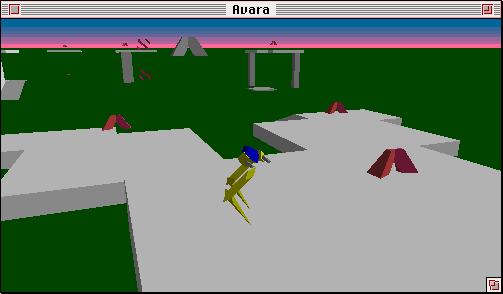
\includegraphics[width=\textwidth]{img/03.png}
\end{center}

The Game window is where your view of the Avara world is displayed. It is re-sizable and you can grow or shrink this window to any size, even to the full size of your monitor. Avara automatically sizes the objects in the scene to the proper scale. Though the window can be made both taller and wider, it is the width of the window that determines the scale of the scene.

The size of this window can affect the performance of Avara. For some Macintoshes, a smaller Game window can lessen the load on the processor and improve the quality of gameplay.

For more information on improving gameplay, see Chapter 14, \textit{Optimization and Troubleshooting}.


\section{Configuring Avara}
\rule{5.5cm}{.15pt}\\
\rmfamily\textit{The Nuts and Bolts}

\subsection{Game Options}
\begin{center}
	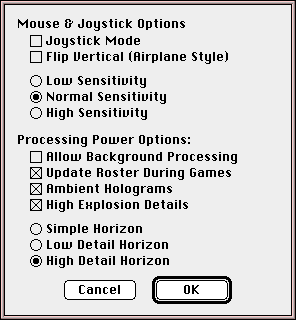
\includegraphics{img/08.png}
\end{center}

\subsubsection{Mouse and Joystick Options}
\textbf{Joystick Mode}: Selecting this option changes the way that Avara takes input from your pointing device. With this option selected, Avara interprets the starting position of your mouse to be ``home'' or ``center''. Deflecting your mouse from its home position will cause the pod of the HECTOR to begin moving in the direction of the deflection. Returning your mouse (or other pointing device) to the home position stops the pod from moving. In technical terms, your mouse normally controls the position of the pod. With this option selected, it controls the velocity of the pod.

\textbf{Flip Vertical (Airplane Style)}: By default, Avara raises the head of your HECTOR when you push the mouse ``up'' or away from you. Selecting this option changes the way that Avara interprets mouse input so that pushing the mouse ``up'' tilts the head of the HECTOR downward. Users who are familiar with flight simulators may prefer this mode.

\textbf{Sensitivity}: Select Low, Normal, or High to set Avara's sensitivity to the movements of your mouse.

\subsubsection{Processing Power Options}
Selecting these options will increase the load on the processor of your Macintosh. Users with less powerful computers should consider leaving these options unselected to improve gameplay.

\textbf{Allow Background Processing}: When this option is selected, Avara will allow other applications that may be running on your Macintosh to share the processor. On less powerful Macs, selecting this option can make gameplay ``jerky'' if you are running other applications. You will almost always want to leave this option off when you play Avara as it is the one thing that can make Avara slow on any Mac. This is particularly important when you play Avara over a network.

IRC users should note that if this option is not selected when playing Avara, their client may ping out.

\textbf{Update Roster During Games}: When this option is selected, Avara will update the display in the Roster window while the mission is running.

\textbf{Ambient Holograms}: When this option is selected, Avara will draw any ambient holograms that are included in a mission.

\textbf{High Explosion Details}: When this option is selected, Avara will increase the detail of explosions in the game.

\textbf{Horizon Detail}: Higher levels of detail will give a smoother color gradation between the ground and the sky. At the Simple Horizon setting, no gradation is shown.

For more information, see Chapter 14, \textit{Optimization and Troubleshooting}.

\subsection{Sound}
Avara allows you to determine where and how the audio output of the game is played. To control where Avara sends the audio output of Avara, select one of the first four options in the \textbf{Sound} menu. These are:

\textbf{Mute}: Turns off all sound. Selecting Mute can help improve the performance of Avara. This option should be considered a last resort, as there are less drastic ways to reduce the additional load that sounds place on your Mac's processor.

\textbf{Monophonic}: Sets sound to be monophonic, rather than stereo.

\textbf{Stereo Headphones}: Selecting this option will decrease the stereo separation to suit listening with headphones.

\textbf{Stereo Speakers}: Selecting this option will provide increased stereo separation to allow for more realistic sound over stereo speakers.

For more information, see Chapter 14, \textit{Optimization and Troubleshooting}.

\subsection{Sound Options}
\begin{center}
	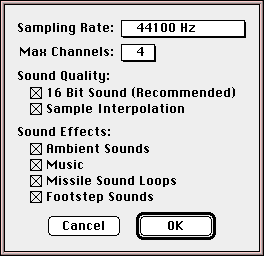
\includegraphics{img/09.png}
\end{center}

Additional sound options can be set in the Sound Options dialog window. To set these options, select \textbf{Sound Options} from the \textbf{Sound} menu.

\subsubsection{Sampling Rate}
This pop-up menu allows you to set the sound sampling rate Avara will use. Higher sampling rates produce higher quality sound, but also increase the load on you Macintosh's processor. On slower Macs, we recommend 11kHz as the sampling rate. If you have the sampling rate for your Mac set in your \textbf{Sound} control panel, be sure not to set Avara to a higher rate. For best performance, use a whole fraction of the rate that is set in your \textbf{Sound} control panel.

\subsubsection{Max Channels}
This pop-up menu allows you to set the maximum number of sound channels that Avara will use. Using more channels will increase the load on your Macintosh's processor.

\subsubsection{Sound Quality}
\textbf{16-Bit Sound (Recommended)}: When this option is selected, and if your Macintosh supports it, Avara will use 16-bit sound to offer higher fidelity. If not selected, Avara uses 8-bit sound.

\textbf{Sample Interpolation}: When this option is selected, Avara uses sample interpolation to increase the quality of the sound in the game.

\subsubsection{Sound Effects}
Each of the options below provides a richer sound environment when playing Avara, but also increases the load on your Macintosh's processor. If you are having performance problems, consider unselecting some or all of these options.

\textbf{Ambient Sounds}: When this option is selected, the ambient sounds contained in a mission are played. This option provides a richer sound environment in Avara.

\textbf{Music}: When this option is selected, any music that is included in a mission will be played. None of the missions that come with Avara contain music, but Avara allows third party mission designers to include music in their missions.

\textbf{Missile Sound Loops}: When this option is selected, Avara will continue to play missile sounds as long as the missile is still flying. When this option is not selected, you will hear a shorter duration sound effect.

\textbf{Footstep Sounds}: When this option is selected, Avara will play the sound of the HECTOR's footsteps.

For more information, see Chapter 14, \textit{Optimization and Troubleshooting}.


\section{The H.E.C.T.O.R.}
\rule{5.5cm}{.15pt}\\
\rmfamily\textit{Your craft in this new world}

\begin{center}
	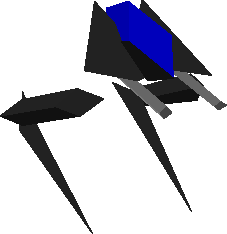
\includegraphics{img/10.pdf}
\end{center}

The vehicle you control in the world of Avara is a \textbf{H}ostile \textbf{E}nvironment \textbf{C}ombat and \textbf{T}ransport \textbf{O}perations \textbf{R}emote unit, affectionately known as the \textbf{H.E.C.T.O.R.} The HECTOR stands two meters high and is equipped with an array of weapons, a scout, and a video camera so that you can see things from the scout's point of view.

HECTORs come in three hull types, Light, Medium, and Heavy. A heavier hull is better shielded and can carry more weapons, but it moves more slowly and can not jump as high. Each has its advantages and disadvantages, and some missions or playing styles may favor a particular configuration. You can change the hull type and weapon configuration of your HECTOR before you load each mission.

Your HECTOR is protected by shields. If you are hit by an opponent's fire, your shields will be depleted. If the strength of your shields is reduced to zero, your HECTOR is destroyed. Damaged shields can be recharged and the HECTOR does this automatically, but recharging takes time, so it is wise to keep track of your shields!

The HECTOR carries a store of energy that it uses to power your plasma cannons and to recharge your shields. The rate at which your shields and cannons are recharged depends on how much energy you have in your store. The HECTOR can generate energy to replace what it uses, but it does this slowly. Conserving energy is an important part of playing Avara well.

\subsection{Movement}
The HECTOR moves a bit like an ostrich. It can walk forward or backward, turn in place, turn while walking, crouch down, and jump. The head, or ``pod'', moves independently of the rest of the HECTOR and can swivel left, right, up, or down.

Use the ``Forward'', ``Reverse'', ``Left'', and ``Right'', keys to walk around. Holding down the Jump key will cause your HECTOR to crouch, and to jump up when the key is released. The ``Vertical Motion'' key lets you raise or lower the stance of your HECTOR. Moving the mouse while holding this key down allows you to change the height at which your HECTOR stands. When you release the ``Vertical Motion'' key, your HECTOR stays at the height you set. Keep in mind that, as HECTORs go, lower is slower. It's hard to walk when crouched down!

Movement of the head is always controlled with the mouse. You can turn the head to look up, down, left or right. To either side, the head can turn approximately 100 degrees from center. Vertically, the head can move about 60 degrees from center. When you move the mouse, your head will move and your view will change in the Game window. The free movement of the head means that the direction you are looking isn't always the direction you are facing. The black ``V'' on your display is used to indicate where ``forward'' is, and this is the direction you will move when you walk forward.

\subsection{Your View from the HECTOR}
Controlling what you see is a critical part of Avara. In addition to using the mouse, you also have keyboard controls that allow you to glance left or right, to zoom in on a distant object, or to aim forward.

With the ``Glance Left'' and ``Glance Right'' keys you can make the camera in the pod of your HECTOR swing to the left or right without moving the mouse. As long as the key is held down, the camera stays turned to the side. When you release the key, the camera swings back to its normal position in the pod.

You are also able to zoom your view in and out by using the ``Zoom In'' and ``Zoom Out'' keys. This allows you to inspect objects that are far away. While you are zoomed in, your view will be very sensitive to mouse movements.

If you become disoriented and lose your sense of which way is forward, use the ``Aim Forward'' key. This will bring the head of your HECTOR back to its natural center.

The ``View Range'' key allows you to control how Avara handles the viewing of distant objects. On a slower Macintosh, it may help to have Avara not draw objects that are very far away. The ``View Range'' key will toggle Avara between Short View range and Long View range. In Short View range, distant objects are ``clipped'' from your view. Avara sends a message to the console of your Instrument window when you change your View Range.

\subsection{The Scout}
Your HECTOR comes equipped with a scout. The scout has a camera mounted in it and can serve as your ``eye in the sky'' as you check out the lay of the land.

When you start a mission, the scout is tucked away in your HECTOR. The ``Scout Control'' key is used to release or recall your Scout. When your scout is released, it hovers behind you. As you move, the scout will follow. You can use the ``Scout View'' key to switch between your view from the HECTOR and the scout view.

For more information on the scout, see Chapter 8, \textit{Denizens of Avara}.

\subsection{Weaponry}
Your HECTOR is armed with plasma cannons, guided missiles, grenades, and energy boosters. There is a limit to how much each hull type can carry, and some missions may limit your weapon load. Keep in mind that carrying more weapons means increasing the total weight of your HECTOR. A lighter HECTOR can move faster and jump higher, so be sure to arm your HECTOR efficiently.

Your current stock of weapons is displayed in the Instrument window, with each band of blue representing one missile, one booster, or two grenades.

\begin{center}
	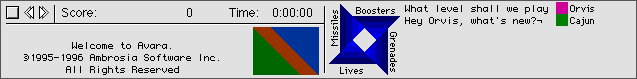
\includegraphics[width=\textwidth]{img/07.png}
\end{center}

Some missions have weapon ``power-ups'' in them that allow you to replenish the store of weapons in your HECTOR.

\subsubsection{Plasma Cannons}
Two plasma cannons come standard with your HECTOR. They are fixed to the pod of your HECTOR and are aimed by moving the head. The green brackets on your display show you the aiming points of your cannons. Your plasma cannons are fired by pressing the mouse button or by using the ``Fire Weapon'' key on the keyboard.

When you fire your plasma cannons, their charge is depleted. Your HECTOR uses its energy store to recharge them, and there is a minimum charge necessary before they will fire again. Keep in mind that the damage a plasma blast will do is related to the charge on the weapon when it is fired. You can use the Instrument window to keep track of the charge on your plasma cannons.

\subsubsection{Guided Missiles}
There are three steps to using Guided Missiles: arming, aiming, and firing. When you press the ``Arm Guided Missile'' key, your HECTOR takes a missile from its store and mounts it in firing position. When a missile is mounted, your plasma cannon sight changes to a missile sight. To lock a missile onto a target, move the sight over the target. When a missile is locked on, a small red ``X'' will appear on the target. To fire the missile, press the mouse button or use the ``Fire Weapon'' key.

If you decide not to fire the missile, press the ``Arm Guided Missile'' key again and your HECTOR will unmount the missile and return it to your store.

\subsubsection{Grenades}
The process of firing a grenade is similar to that of the guided missile. When you press the ``Arm Grenade'' key, your HECTOR takes a grenade from its store and mounts it in firing position. When a grenade is mounted, your plasma cannon sight changes to a grenade sight. The sight indicates where the grenade will fall, so use the mouse to move the sight onto your target. To fire the grenade, press the mouse button or use the ``Fire Weapon'' key.

If you decide not to fire the grenade, press the ``Arm Grenade'' key again and your HECTOR will unmount the grenade and return it to your store.

For more information, see Chapter 12, \textit{Tips, Tactics, and Strategy}.

\subsubsection{Energy Boosters}
Energy Boosters are very handy in a tough battle. A Booster will quickly recharge your energy, shields and plasma cannons. Although your HECTOR recharges your shields and cannons automatically, you may find yourself in a position where you need them recharged quickly. In these situations, pressing the ``Energy Boost'' key will put your HECTOR back in top fighting form.


\section{Denizens of Avara}
\rule{5.5cm}{.15pt}\\
\rmfamily\textit{You never know who you'll meet.}

\subsection{The Scout}
\begin{center}
	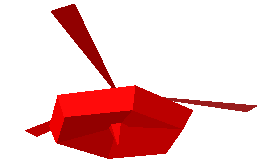
\includegraphics{img/11.pdf}
\end{center}

Your HECTOR comes equipped with a remote video camera attached to a small hover vehicle. The ``Scout Control'' key acts as a toggle, and will release or recall your scout. When you release the scout from your HECTOR, it takes up a station above and behind you. When you move, the scout follows you around. Your scout keeps its camera trained on you, and you can switch to the view from your scout at any time. The ``Scout View'' key toggles the view between your scout and your HECTOR. If you switch to ``Scout View'' when your scout is not released, your HECTOR will automatically launch your scout.

If you like, you can change the position of your scout relative to your HECTOR by using the ``Scout Control'' key in combination with the direction keys. In the standard keyboard mapping these combinations are attached to the arrow keys. If you want your scout to keep a station to your right rather than behind you, simply tap the right arrow. Your scout will move off to the right of your HECTOR and stay ``on station'' as you move. Likewise, the up arrow will make your scout keep a station in front of your HECTOR.

You can use the ``Scout Control'' key in combination with the ``Aim Forward'' key to force your scout to stay in one place. The camera in your scout will continue to track your HECTOR, but the scout will remain in place until you recall it by using the ``Scout Control'' key.

Your scout is hardy, but it isn't indestructible! Hostile units can target your scout, and if it takes enough damage it will be destroyed. If you lose your scout, you won't get another in that mission.

\subsection{UFOs}
\begin{center}
	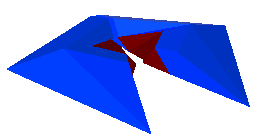
\includegraphics{img/12.pdf}
\end{center}

Some Avara levels are populated with UFOs. UFOs deliver a nasty wallop, so it is wise to have a healthy respect for them! Although their energy bursts are powerful, they have a hard time hitting moving targets. It is best to keep moving when you are being attacked by a UFO. Try using missiles against them. Once the missile is locked on the target, you can fire and then concentrate on dodging!

\subsection{Guards}
\begin{center}
	
\includegraphics{img/13.pdf}
\end{center}

A Guard is a gun emplacement. It tracks targets within its range, and fires a nasty bolt of energy whenever it has a clear shot. Guards fire fairly quickly and pack a big punch, but they turn slowly. When you are in range of a guard, it is best to step lively!

\subsection{Parasites}
\begin{center}
	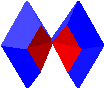
\includegraphics{img/14.pdf}
\end{center}

Parasites lead a bizarre existence. Their sole purpose in life is to find a HECTOR and feed on its energy. If a parasite sees you, it will move slowly toward your HECTOR and try to attach itself to your hull. If a parasite successfully attaches itself to your HECTOR, it will drain some of your energy. When it is full, it will explode with joy!

\subsection{Transporters}
\begin{center}
	
\includegraphics{img/15.pdf}
\end{center}

Transporters are simple things. Entering a transporter takes your HECTOR some place else. The fun is that sometimes you don't know where you will go!

\subsection{Switches}
\begin{center}
	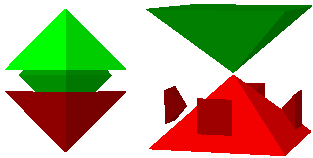
\includegraphics{img/16.pdf}
\end{center}

Switches can be used to control actions in an Avara mission. To activate a switch, just shoot it with your Plasma Cannon. Keep an eye on the scene, since you will want to know what the switch does.

\subsection{Mines}
\begin{center}
	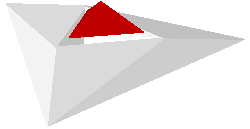
\includegraphics{img/17.pdf}
\end{center}

Mines in Avara work as you might expect them to, they blow up!

\subsection{HECTORs}
\begin{center}
	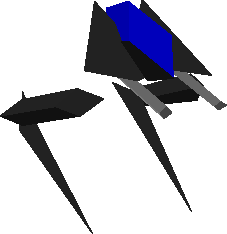
\includegraphics{img/10.pdf}
\end{center}

In Network Avara, you interact with the HECTORs of the other players.

Other HECTORs that are the same color as yours are on your team. You should work with them to reach your goal, or to destroy the other team.

Any HECTOR of a color different from yours is not on your team. This doesn't necessarily make it your enemy, but that might just be the case.

Not all network games of Avara are ``blow the other guy away'' games. Some missions are set up to be cooperative, and some are competitive in a different way.

For example, you can play ball games in Avara. In ball game missions, the object is to score points by getting the ball in the goal. You can move a ball by shooting it, or you can pick it up and run with it. To release a ball, or any object you are carrying, hit any ``load weapon'' key.

Avara is an incredibly rich environment, and the type and style of missions that can be created is limited only by the imagination of the mission designer.

For more information on designing levels for Avara, see the section on Creating New Levels in Chapter 13, \textit{Avara Extras}.

\begin{center}
	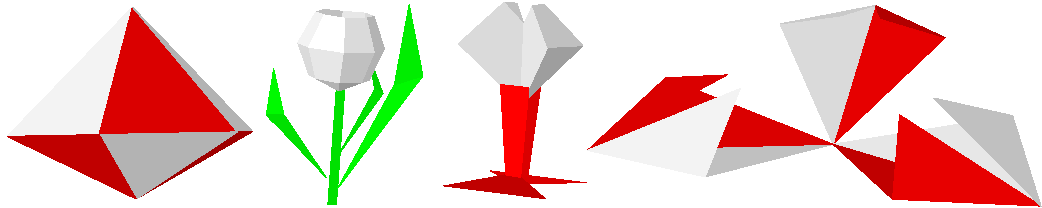
\includegraphics[width=\textwidth]{img/18.pdf}
\end{center}

\subsection{Objects}
The world of Avara is made up of objects. Walls, doors, ramps, flowers, balls---there is no limit to what can be created. Particularly in the solo missions, much of what you do is to interacting with the objects in the level. As you work your way toward the goal of a mission, keep in mind that objects can be moved, carried, activated, or destroyed. Any one event in Avara can trigger something else. Walking across an open space might open a door, a platform might move vertically like an elevator, or destroying a block might unleash a hoard of UFOs!


\section{Network Avara}
\rule{5.5cm}{.15pt}\\
\rmfamily\textit{Playing others over a network}

As great as Avara is as a single-player game, it can be even better when played over a network. Avara allows up to six players in a single game, but keep in mind that the type and quality of network connection you use will affect the gameplay.

Avara can be played over an AppleTalk network, or over the Internet. The following sections describe the basics of playing a network game. For specific information on playing Avara over an AppleTalk network, see Chapter 10, \textit{AppleTalk Avara}. For instructions on playing Avara over the Internet, and some basic steps you can take to optimize performance, see Chapter 11, \textit{Internet Avara}. Further details about optimization can be found in Chapter 14, \textit{Optimization and Troubleshooting}.

\subsection{Playing a Network Game}
Up to six players can participate in a networked game. Avara allows the players to battle for a common goal, to set up competing teams, or to play every HECTOR for itself!

Avara can be played over an AppleTalk network, or over the Internet. A network game of Avara begins by having one person start up Avara and create a ``server.'' Once a server is running, up to five other players can connect to the server as ``clients.''

Avara creates a true network among the connected machines. That is to say, each Macintosh communicates directly to every other Mac in the network. Because of the way a network game of Avara is set up, being the ``Server'' machine gives no real network advantage. All the Macs communicate on an equal basis. The person playing on the server does have control over some of the options that can be set in a network game, and is responsible for keeping the Avara network up. If the person running the server quits Avara, the network is shut down.

When Network Avara is running, it is ``frame synched.'' This means that Avara forces every machine on the network to animate the action at the same frame rate. The game can only run as fast as the slowest Macintosh in the Network, so making sure that everyone in the game is set up properly is important. For tips on optimizing performance, see the information in this chapter and Chapter 14, \textit{Optimization and Troubleshooting}.

You can only play Avara other people who have the same version that you do. If in the future an updated version of Avara is released, you will have to get the new version to be able to play with others who have the new version. For information on keeping up with the latest news from Ambrosia, see the section on the Announcement List in Chapter 16, \textit{Registration, Contact Information, and Credits}.

\subsection{Loading a Mission in a Network Game}
Missions load the same way in a network game of Avara as they do in a solo game. To load a mission, just click on it in the Player window. To display a new set of missions, select \textbf{Open\dots} from the \textbf{File} menu and then select any available level file from a folder or drive on your Macintosh. If the ``Server Options'' are set to allow it, any player in the game can load a mission.

It is important to note that in order for a mission to load, each player in the game must have that mission file on their Macintosh. Avara does not send missions across the network.

\subsection{The Roster Window Revisited}
The Roster window is where you organize players into teams for a network game. Each Player Field on the ``All'' tab can be dragged to rearrange the order of the players on the tab.

To create teams, simply set the colors of the individual players. All players of the same color are on the same ``Team.'' Avara will keep track of both individual and team scores on the ``Results'' tab of the Roster window. Once the mission is started, the teams can not be rearranged for the duration of that mission.

The status of each player is displayed on the ``All'' tab, and on the individual ``Player'' tabs.

\subsection{Chatting}
\subsubsection{Before or Between Missions}
Players in a network Avara game can communicate with the other players in the game by typing. When a mission is not running, all you need to do is type what you want to say. The text you type will scroll across the various tabs of the Roster window, and along the Instruments window. The ``Chat'' tab of the Roster window organizes the text from all the players in an ``IRC'' fashion. In all the other places that text is displayed, it simply streams across the field as it is typed. Hitting the \textbf{\keys{Return}} key as you type will send your current block of text to the ``Chat'' tab, but in all the other fields an actual Return character is displayed.

You can send an audible ``beep'' while chatting by typing a \textbf{\keys{Ctrl-G}} character. To set the sound you will hear when a \textbf{\keys{Ctrl-G}} character is sent, select \textbf{Bell \keys{Ctrl-G}} from the \textbf{Sound} menu and choose one of the system sounds displayed in the pop-up menu. If you do not wish to hear \textbf{\keys{Ctrl-G}} sounds, select \textbf{No Sound} from the \textbf{Sound} menu.

\subsubsection{Chatting While a Mission is Running}
When a mission is running, you use the keyboard to control the HECTOR. To chat while on a mission, use the ``Message Mode'' key. When you hit the ``Message Mode'' key, Avara begins sending the keystrokes you type as chat text. Hitting the ``Message Mode'' key one more time will turn off message mode and allow you to control your HECTOR again.

\subsection{Uh Oh, I Lost}
Even the greatest players sometimes lose. If you are playing in a network game, and you lose your last HECTOR, you can use the ``Abort'' key to quit out of the mission while still remaining connected to the server. Just hold down your ``Abort'' key until your status in the Roster window changes from ``active'' to ``connected''. If you are the Server, using ``Abort'' will allow you to do other things while the clients on your server finish up their game. So if you don't win in a network game, don't quit. Abort out of the mission and plot your revenge while you wait for the others to finish!

\subsection{Setting Your Server Options}
\begin{center}
	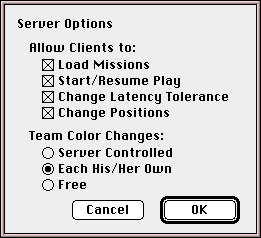
\includegraphics{img/19.png}
\end{center}

In a network, the player who first started Avara is the server. This player can set the ``Server Options'' for the game. None of these options in any way affects the actual network; they simply allow (or disallow) clients to make changes in the configuration of the game. To bring up the ``Server Options'' dialog box, select \textbf{Server Options\dots} from the \textbf{Network} Menu.

\subsubsection{Load Missions}
Selecting this option allows clients to load new missions. When this option is not selected, only the server can load new missions.

\subsubsection{Start/Resume Play}
Selecting this option allows clients to pause the game, and to restart it after a pause. If this option is not selected, only the server can pause Avara.

\subsubsection{Change Latency Tolerance}
Selecting this option allows clients to select a new Latency Tolerance for Avara. When this option is not selected, only the server can change the Latency Tolerance. For more information on Latency Tolerance, see the section on Latency Tolerance in Chapter 11, \textit{Internet Avara}.

\subsubsection{Change Positions}
Selecting this option allows clients to change the positions of the players on the ``All'' tab in the Roster window. When this option is not selected, only the server can change the order of players in the Roster window.

\subsubsection{Team Color Changes}
This option determines who can change the colors of HECTORs in the game. If Team Colors are \textbf{Server Controlled}, only the server can set the colors (and therefore the teams) of the individual players. Setting this option to \textbf{Each His/Her Own} allows players to individually select their color or team. Setting this option to \textbf{Free} allows any player to set the color and team of any other player in the game.

\subsection{Avara Etiquette}
Network Avara is more than just a game, it is a community. Avara comes with chatting ability built right in, so when you first join a game, say ``Hi.'' If the other players are waiting, chat with them. They may even talk a little friendly trash as a pre-game warm up. If the players already connected are on a mission, they won't want to chat with you right away. They're not being rude, they're just busy. Avoid selecting their player tabs, as the game may slow down while you download their player pictures. When the mission is over, they will return your greeting.

Once you're in, it's best to leave the loading of missions to the person who started the server. Also, the player on the server may wish to make up the teams his or herself. The players may discuss network settings, and this is a good time to get advice on what settings to use in the game.

While you are playing, try to give the other players a little warning if you have to pause the game for some reason. It's frustrating to have the game pause frequently in a heated battle! More importantly, you should ask to make sure that everyone is ready before you resume the game. It gives the other players a chance to finish what they were typing, and to get their fingers back onto the right keys.

If you start your own server, be sure to add an invitation message so that others who see your game on the Tracker will know what sort of game will be played. You may want to consider freeing up some of the ``Server Options.'' It is polite to allow other players to pick their own colors, and to pause or resume the game.

If you have to go away for a short time, but want to leave the server up, you can let other players know by adding (away) to your name in the Player window. Just change it back when you return.

Last but not least, always remember there are real people with real feelings on the other end of your network.


\section{AppleTalk Avara}
\rule{5.5cm}{.15pt}\\
\rmfamily\textit{Playing over a local AppleTalk network}

\subsection{Setting Up an AppleTalk Game}
\subsubsection{What you need}
All you need is two or more Macintosh computers connected with an AppleTalk network. Either Ethernet or LocalTalk will work. With AppleTalk, you can take your Macintosh over to your friend's house, plug in a LocalTalk cable, and fire up Avara!

Running Avara on an AppleTalk network requires that all the Macintoshes in the game have Program Linking turned on. To turn on Program Linking, select the \textbf{Sharing Setup} control panel. If Program Linking is currently stopped, click on the ``Start'' button below the Program Linking icon. Once Program Linking is turned on, select the \textbf{Users \& Groups} control panel. To allow any Macintosh on your local network to connect to your machine, double-click on the ``Guests'' icon and make sure that Program Linking is turned on for guests. If you wish to limit who can connect to your Macintosh, you will need to create a new user or group for those who you wish to allow to connect. See the \textbf{Apple Guide} or the documentation that came with your Macintosh for instructions on setting up new users or groups.

\subsubsection{Connecting to an AppleTalk Server}
To connect to an Avara Server running on an AppleTalk network, select one of the AppleTalk options from the \textbf{Network} menu and click on the ``Connect to Server\dots'' button in the Player window. This will bring up a dialog box that will allow you to select the machine to which you wish to connect. Avara does not look for games on your AppleTalk network, so you must either know the name of the machine you wish to connect to or browse through the listed machines to find one that is running Avara. When you find a computer that is running an Avara Server, click on ``OK'' to join the server. If you are on a larger network that has multiple AppleTalk Zones, you may select a Macintosh in another zone by first selecting that AppleTalk Zone, and then selecting a Macintosh that is running Avara.

\begin{center}
	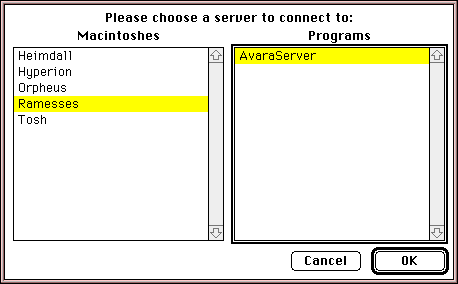
\includegraphics[width=\textwidth]{img/20.png}
\end{center}

\subsubsection{Creating an AppleTalk Server}
If you wish to start your own Avara Server, select one of the AppleTalk options from the \textbf{Network} menu and click on the ``Start Server\dots'' button in the Player window. Your server is now running, and any Macintosh that is connected to your AppleTalk network can now join your game by following the instructions in the section above.


\section{Internet Avara}
\rule{5.5cm}{.15pt}\\
\rmfamily\textit{Playing Avara over the Internet}

\subsection{Setting Up an Internet Game}
\subsubsection{What You Need}
You will need a Macintosh with a link to the Internet. This means either a Macintosh with a direct Internet connection (like those found at many schools and businesses), or a Macintosh with a modem connection to an Internet Service Provider (ISP). Some commercial network services do not offer direct Internet access. You will not be able to play Avara over these networks.

Please keep in mind that the quality of your Internet game will depend on MANY factors including but not limited to the speed, load and/or quality of:

\begin{itemize}
	\item any modems in the network
	\item your local network
	\item the Internet connection at your ISP
	\item the Internet connection at the ISPs of all other players in the game
	\item your Macintosh, or the Macs of any of the other players in the game
\end{itemize}

As an example, suppose you want to play Avara with a friend in another city. Consider the path the network information must travel along. Starting with your computer, the information has to go through your modem and over the local phone lines to a modem at your ISP. Your ISP then sends it out through their gateway to the Internet at large, where anything can happen. After it finds its way over the Internet to your friend's ISP, it is then passed through a modem there and over the phone lines in your friend's city to the modem he has at home, and finally to his computer. A network problem could occur at any one of those points which would make Avara very difficult to play. The Internet might just be having a bad day.

Don't lose heart though. Things are not that gloomy. The author of Avara, who lives in Finland, has played good-quality games with players in the United States over his 14.4 modem. Many other players have had wonderful success playing from home. The point is that there are many factors involved in creating a good Internet link, some of which you cannot control.

\subsubsection{The Avara Tracker}
Ambrosia Software runs an Internet Avara Tracker in its office to make finding and joining an Internet game of Avara easy. When anyone starts up an Internet Avara Server, they have the option of notifying the Tracker. If you notify the Tracker, information about your game (including the IP address) is sent to the Tracker at Ambrosia, where it is made available to anyone who is looking for a game of Avara.

To find an Avara game on the Internet, just send a query to the Tracker. The Tracker will send you information listing all of the games that are currently registered. You can query the Tracker from within Avara, or you can use the MicroTracker that is included in the Avara distribution. See Chapter 13, \textit{Avara Extras} for information on the MicroTracker.

At this time, there is only one Avara Tracker. In the future, it is possible that additional trackers will be running. In this is case, both the ``Look for Server\dots'' dialog and the ``Start Server\dots'' dialog allow you the option of registering your game at a different tracker by entering the IP name or number in the appropriate box. Additional tracker addresses can be kept in a Hotlist. To use the Hotlist, simply click on the arrow to the right of the tracker address. The domain name address of the Avara Tracker at Ambrosia is: \textbf{\texttt{tracker.Avara.com}}

\subsubsection{Connecting to an Internet Server}
To connect to an Avara server running somewhere on the Internet, select the \textbf{TCP/IP} option in the \textbf{Network} menu and click on the ``Connect to Server\dots'' button in the Player window. This will bring up the ``Connect to Server\dots'' dialog window.

\begin{center}
	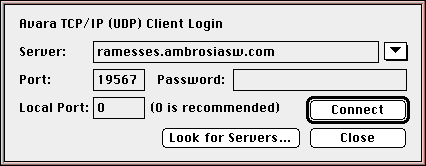
\includegraphics{img/21.png}
\end{center}

If you know the IP address or IP number of the machine you wish to connect to, simply type it into the ``Server'' box. If the game you wish to connect to is protected by a password, enter it into the ``Password'' box. In some situations, it is possible that you will need to set a separate port for Avara to run on, but in most cases the default port will be the one you want. See Chapter 14, \textit{Optimization and Troubleshooting} for more information on ports.

If you find that you connect frequently to a particular address, you can add that address to the Hotlist. To add an IP address to your Hotlist, click on the arrow to the right of the address and select ``Add to Hotlist'' from the pop-up menu. To remove an IP address from your Hotlist you should select the address, click again on the arrow to the right, and select ``Remove from Hotlist.''

When you have entered the information that Avara needs, click on the ``Connect'' button. Avara will then attempt to connect to the IP address of the server you have specified.

If you don't know of any machines that are running Avara, don't worry. Avara also lets you check to see if there are any games available on the Internet. To find other Internet Servers, click on the ``Look for Servers\dots'' button in the ``Connect to Server\dots'' dialog window.

This brings up a window that allows you to query the Avara Tracker running at Ambrosia. Simply click on the ``Search'' button to query the Avara Tracker. It will return to you a list of games that are currently registered on the Tracker. To get more information on any of the games listed, select it from the list with a single click. Additional information will appear in the box on the right.

\begin{center}
	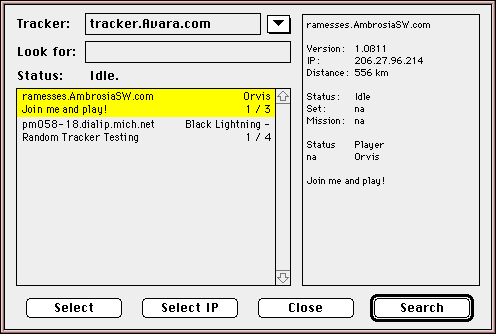
\includegraphics[width=\textwidth]{img/22.png}
\end{center}

Each time you click on the ``Search'' button, updated information from the Tracker is displayed in your window.

To help sort through the games on the Tracker, you can use the ``Look for'' box to search for particular games. Just type words that describe who or what you are looking for in the ``Look for'' box and click on the ``Search'' button. The Tracker will check your criteria against the list of registered games and send you a list of all the games that match your criteria. For example, if you enter \textbf{\texttt{college.edu}} and click on the ``Search,'' the Tracker will send you the list off all the registered games that have ``college'' and ``edu'' in any of the fields. The Tracker looks at all information for each registered game, so you can search for a particular player by typing that player's name in the ``Look for'' box. The Tracker is not case sensitive and will search for multiple criteria, just separate each word with a space. Searching for \textbf{\texttt{Berserkir Ambrosia}} will return a list of all the games started by anyone named ``Berserkir'' at any place named ``Ambrosia.''

If you do a search on help (by typing ``help'' in the ``Look for'' box), the Tracker will display a short introduction to using the search capabilities of the Tracker.

If the Tracker doesn't see any games that match your criteria, it returns ``No Matches.'' If this happens, try using a different criteria, or no criteria, in the ``Look for'' box. If there are no games registered on the Tracker, any search will return ``No Games.'' In this case, you should start your own server!

To join a game, select the one you are interested in and click on the ``Select'' or the ``Select IP'' button. This will return you to the ``Connect to Server\dots'' dialog and automatically enter the information from the game you selected. Click on the ``Connect'' button to join the server.

If there are no servers listed on the Tracker, you can start your own. It is very possible that somewhere in the world, someone else is also looking for a server! The following section shows you how to start your own Internet Avara Server.

\subsubsection{Creating an Internet Server}
If you wish to start your own Internet Avara Server, select the \textbf{TCP/IP} option from the \textbf{Network} menu and click on the ``Start Server\dots'' button in the Player window. This will bring up the ``Start Server'' dialog window.

\begin{center}
	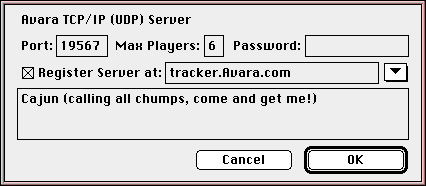
\includegraphics{img/23.png}
\end{center}

If you wish to limit the number of players that can be in your game at any one time, enter the number in the ``Max Players'' box. In all cases, six players (including you) is the limit in any Avara game.

If you wish to set a password for your server, enter it in the ``Password'' box. If your game is protected with a password, other players will have to enter it when they attempt to join your server.

If you want to register your game with the Avara Tracker, select the check box to the left of the ``Register Server at'' box. This ensures that your Avara game will be listed on the Tracker, and can be found by anyone on the Internet who is looking for a game.

You can type a message in the box at the bottom of the window. This message will be displayed to anyone who queries your server on the Tracker.

When you have configured your server, click the ``OK'' button. This will start your Avara server. If you have selected the ``Register Server at'' box, your server information will now be sent to the Tracker.

Your server is now running. If you have notified the AvaraTracker, any other Macintosh that is connected to the Internet can now find and join your game by following the instructions in the section above.

Avara can be set to notify you if anyone joins the game you are in. The \textbf{New Arrivals Alert} item in the Sound menu allows you to set a sound to be played whenever anyone joins the game you are in. Simply select any of the system sounds listed in the pop-up menu, or select \textbf{No Sound} if you do not wish to be notified.

\subsubsection{Reconfiguring your Internet Server}
If you need to change the configuration of your Avara Server, select \textbf{Reconfigure Server\dots} from the \textbf{Network} menu. This will bring back the ``Start Server'' window, and allow you to change the options you selected previously.

\subsection{Getting the Most from Your Network}
Avara allows you to change the way it uses the available network resources. Tuning the network settings of Avara is an important part of playing a smooth network game.

\subsubsection{Latency}
Latency is a measure of the time between when your computer sends out network information and when another computer receives it. Every device in the chain that makes up your network adds some latency. In a network game, Avara is trying to keep everyone ``on the same page,'' and it has to do a balancing act between providing quick response to your controls and making sure that the other computers on the network keep up with whatever you are doing.

The way that Avara compensates for latency is to create an artificial delay (a ``Latency Tolerance'') in the way it responds to your controls. It slightly delays your actions to make sure that the rest of the computers in the game can coordinate your actions with those of the other players. Driving the HECTOR with a very high latency tolerance is a bit like steering a large boat, you turn the wheel and then wait a bit for the boat to respond.

If all the network connections in your game are good, you should be able to play with a very low latency tolerance (or ``LT''). If there is some delay, you can either set a higher LT or have Avara do it for you.

To have Avara decide what LT is best, select \textbf{Automatic Latency} from the \textbf{Network} menu. As your game runs, Avara will adjust the LT. If Avara makes a change in the LT, a message will be sent to to the Instrument window to let you know what the new value is.

You can also force Avara to run at a specific LT. To set a specific LT for Avara, select \textbf{Latency Tolerance} from the \textbf{Network} menu and choose the LT setting you want from the pop-up menu that appears.

If you force Avara to run at a lower LT than the network can keep up with, you may experience ``jerky'' game play. Avara will freeze the game for a moment to allow all the computers to catch up with everything that is going on in the game.

\subsubsection{Bandwidth}
Avara can be set to use additional bandwidth to send redundant information across the network. If the network connection between the players in the game is very good, it is not necessary to send redundant information. In this case, a minimal or low bandwidth setting will make for smooth play. However, if some of the network connections in the game are of poor quality, game play can be improved by increasing the bandwidth setting.

To set the bandwidth usage in Avara, select \textbf{Bandwidth Use} from the \textbf{Network} menu and choose the bandwidth setting you want from the pop-up menu that appears.

A good indicator of the quality of your connection to any player in the network can be found on that player's tab in the Roster window. On the right side of a player's tab is a summary of network information, including his IP address, his bandwidth use setting, and a set of estimates that Avara makes about the network between his machine and yours. To get a sense of the connection quality between you and the other player, look at the LT estimates. If there is a large difference between the optimistic LT and the pessimistic LT, your network may be losing information and will benefit from a moderate or high ``Bandwidth Use'' setting.

So why not leave ``Bandwidth Use'' set to high all the time? If bandwidth is used to send redundant information, it can't be used to do other things, like support additional players in a game. More players require more bandwidth because your computer has to send information to all the other players in the game.

For example, if you play from a 14.4 modem, you don't have very much bandwidth to begin with. Asking Avara to send out lots of redundant information may require more bandwidth than you have available, and will actually slow down your game.

In general, faster Internet connections, like ISDN or Ethernet, can benefit more from higher bandwidth usage.

You may have to experiment with different settings to find out what works best for you. Other players in the game may be able to offer helpful suggestions.

For more information on tweaking your network to get better performance, see Chapter 14, \textit{Optimization and Troubleshooting}.


\section{Tips, Tactics, and Strategy}
\rule{5.5cm}{.15pt}\\
\rmfamily\textit{Seminal detritus, with help from Zebetrious}

\subsection{Movement}
Piloting the HECTOR may take a little getting used to at first. The head of the HECTOR moves very freely, so the direction you are looking in is often not the direction you are walking in. Use the large ``V'' on your heads-up display to keep track of which direction you are facing. If you get confused, try using the ``Aim Forward'' key to re-center the head of your HECTOR. The default key for ``Aim Forward'' is \textbf{\keys{2}} on the main keyboard (above the \textbf{\keys{W}}, not on the numeric keypad).

It may also help to watch your HECTOR from your Scout as you move around. For more information about the Scout, see Chapter 7, \textit{The H.E.C.T.O.R.}, or Chapter 8, \textit{Denizens of Avara}.

\subsection{Aiming}
\subsubsection{Plasma Cannon}
Use the brackets on your heads-up display to aim at your target. When the brackets turn from green to red, you are ``on target.'' If your target is moving, you may have to compensate some by leading your target before you fire.

\begin{center}
	
\includegraphics{img/24.pdf}\\
	\sffamily{\footnotesize\textbf{Plasma Cannon Sights}}
\end{center}

\subsubsection{Missiles}
When you arm a missile, your aiming brackets change to a missile sight. Move the sight over your target, and a small red ``x'' will appear on your target. You are now ``Locked On!'' Fire your missile! If your target moves behind an obstacle before you fire, you are still locked on. Your missile can still track the target, even if you can't see it.

\begin{center}
	
\includegraphics{img/25.pdf}\\
	\sffamily{\footnotesize\textbf{Missile Sight and Locked-On indicator}}
\end{center}

If you fire your missile before you have a ``lock,'' it will fly in a straight line until it encounters an obstacle. A missile cannot acquire a target after it has been launched. However, it can still do damage to whatever it hits.

\subsubsection{Grenades}
When you arm a grenade, your aiming brackets change to a grenade sight. Place the sight where you want the grenade to fall, and launch your grenade! Grenades are proximity weapons, so even if you don't hit your target directly you can still cause damage.

\begin{center}
	
\includegraphics{img/26.pdf}\\
	\sffamily{\footnotesize\textbf{Grenade Sights}}
\end{center}

Grenades are launched in an arc, so it is possible to toss grenades over a wall at a target you can't see. The grenade sight will change to indicate that a grenade will land beyond your field of vision.

The motion of your HECTOR affects the path your grenade travels when you fire it. For example, if you are running forward when you fire a grenade, it will fly farther. The grenade sight will move to reflect any change due to the motion of your HECTOR.

\subsection{Incoming!}
Enemy missiles or grenades can be destroyed with a plasma cannon. If you are a good shot, you can blow an incoming weapon out of the sky before it hits you. A particularly nasty trick is to hit a missile or grenade before your enemy fires it. If you shoot a weapon that your enemy has mounted but not yet fired, it will blow up right on his HECTOR!

\subsection{Energy}
Always keep track of your energy. Your energy is used to recharge your plasma cannons and to recharge your shields. Your energy will regenerate, but it does so slowly. If you find yourself low on energy, it might be a good time to play a delaying game. Don't confront an enemy head-on if your energy is low.

If your energy situation is critical, or if you don't have the option to get out of danger quickly, use a booster. A booster will recharge your shields, your plasma cannons, and your energy store. You have a limited number of boosters, so use them carefully. Some missions have energy power-ups that act as boosters.

\subsection{“Machine Gun Syndrome”}
Your plasma cannons need to recharge each time they fire. If you fire before they are fully charged, the damage they can do is reduced. Recharging your cannons takes energy. Consider what happens if you hold down the ``Fire'' key, blazing away at an enemy. You may hit your target a few times with weak shots, but you will also draw down your energy. Sometimes a better tactic is to use your cannons more sparingly. If you make sure of each shot, then each hit will pack a bigger punch. So, aim carefully, make each shot count, and watch those energy levels!

\subsection{Dealing with Missiles}
You never saw him lining up on you, but you hear the result!

\textbf{*SHHhhhhhhhh*}

A missile is locked on and headed your way! Are you dead meat? Should you give up now?

\textbf{NEVER GIVE UP!}

A missile is relentless, but it is also rather dumb. Missiles try to follow the shortest path to their target. They don't worry about intervening structures. Missiles also have a rather large turning radius. If a missile goes whizzing by your head, it can't just stop and spin. It has to turn along a wide arc to try and get back to its target.

Armed with these useful tidbits, there are a few tricks you can use to avoid missiles. If you hear an incoming missile, try heading for a crowded area. Walls, pillars and buildings are your allies. As you weave a path through the obstacles in your way, the missile will readjust its course to stay on target. It won't follow your path, it will try to fly directly at you. If you dodge around a corner at the right time, it will very likely impact harmlessly on the wall you just ducked behind!

But what if you are stuck out in the open? Nowhere to run, baby, nowhere to hide!

You can still avoid the missile with a little good timing. Keep your cool and crouch as the missile bears mercilessly down upon you. Then, at the last instant, JUMP! The missile won't be able to turn fast enough to hit you and will go whizzing on by. If it is coming at you from above, even better! A well-timed jump will cause it to hit the ground and explode harmlessly.

\subsection{I Give Up}
Well, you don't have to give up. If you get lost, trapped, or stuck in a mission, you can use the ``Abort'' key to destroy your HECTOR. If you have lives left, you will get a new HECTOR at the starting point of the mission. You can also use the ``Abort'' key to quit from a mission in a network game of Avara while still staying connected to the Server.

\subsection{Mass vs. Mobility}
Keep in mind that you can configure your HECTOR to suit your own style. If you like to go toe-to-toe with your opponent, you may want to use a Heavy Hull and load it up with ammunition. Remember though, you will not be able to run as fast or jump as high. If you favor maneuverability, try a Light Hull with a lighter load. Some levels may also play more easily with a specific type of setup.

\subsection{Playing with a Teammate}
In network games of Avara, you often have a chance to play cooperatively with another player against another team. The ever-changing environment of Avara means that there are no hard and fast rules for team play, but in general, you should try to work with your teammate without standing right next to him. If you are far away or out of sight of your teammate, you won't be able to help him, and he won't be able to help you. On the other hand, it's also possible to be too close. If you stand right next to each other you not only inhibit your mobility, but you also make an excellent target for an enemy grenade!


\section{Avara Extras}
\rule{5.5cm}{.15pt}\\
\rmfamily\textit{Other goodies}

Ambrosia has included a few additional items designed to enhance your Avara experience:

\subsection{Avara Commuter}

\includegraphics{img/27.png}\\ [0.25em]
Avara Commuter is designed for people who often play Avara on different Macs, such as those in a computer lab at school. Once you have paid for Avara, your copy is personalized with your name (which appears in network games). However, this information is lost when you move Avara to a new computer, which can be cumbersome if you play from a computer lab.

Ambrosia to the rescue! Avara Commuter keeps a copy of your registration information. Running Avara Commuter on a computer in a lab will register your copy of Avara on that computer. It even totes around your preferences file for you! When you quit Avara Commuter, your registration information and your preferences file are removed from the computer.

\subsection{The Avara MicroTracker}

\includegraphics{img/28.png}\\ [0.25em]
The Avara MicroTracker allows you to search for Internet games of Avara without having first to run Avara. To see if any games are currently registered at the Avara Tracker, just run the MicroTracker. It will let you search for Internet games exactly the same way you do in Avara.

If you already have Avara running as a server, you can use the MicroTracker to see what other games are out there without closing the server. Just put Avara in the background and run the MicroTracker.

\subsection{Making Your Own Missions}
With a drawing program and a little imagination, you can create your own Avara missions.

The objects in Avara missions are created as layered drawings saved in PICT files. All you need to create a mission (sometimes called a ``level'') is a color capable drawing program that keeps track of layers.

Most of the missions that come with Avara were created with ClarisWorks, and it is quite likely that your Macintosh already has ClarisWorks installed. (Apple includes it on most of the Macs it sells.) ClarisDraw is a little more powerful, and has some features that make mission design easier.

If you don't have either Claris program, consider using ShareDraw. It is shareware (\$30) and will work just fine as a mission editor. It even sports some features that neither of the Claris programs offer.

You don't need anything more than a drawing program, but if you are ambitious you can create your own sounds or 3D objects for use in your Avara missions.

Avara uses a custom sound format. A program called SoundComp is included in the Avara distribution and is used to convert sounds from SoundEdit format to the Avara format. Many of the sounds that are included in Avara were created with SoundEdit, which is a commercial product. The author of Avara found that Sound Sculptor II (shareware, \$30) was better than SoundEdit in many ways. If you wish to create custom sounds for your missions, Sound Sculptor II is highly recommended.

Avara also uses a custom 3D geometry format. The BSPSplitter program included in the Avara distribution accepts either DXF polygonal models (AutoCAD format) or OFF .geom files (without proper support for color) and converts them to the Avara format. Most of the models in Avara were created with StrataStudio Pro. Some were made with Infini-D. Both of these programs are commercial. Any 3D program that creates DXF models should work, and a shareware program called PatchDance is available (shareware fee is on a sliding scale: \$0--\$75). PatchDance requires a PowerPC and uses Apple's QuickDraw 3D.

With the shareware programs, you have all you need to create your own missions in Avara. Ambrosia is happy to support and promote shareware. If you try these programs and find them useful, please support their authors by paying your shareware fee!

For complete instructions on how to go about creating an Avara mission, please refer to the Avara Level Design Manual in the Avara distribution.


\section{Optimization and Troubleshooting}
\rule{5.5cm}{.15pt}\\
\rmfamily\textit{Getting the best performance}

\subsection{Improving Avara's Performance on Your Macintosh}
If you own the latest and greatest Macintosh, one that is chock-full of processing power and RAM, then this section might not be very interesting for you. Avara will very likely run just fine for you no matter how many options you turn on. However, if you are the proud owner of a more humble Mac, you may wish to browse the section below.

In general, Avara runs best when it has the uninterrupted attention of your Mac. Anything that uses processing power is taking it away from Avara. Improving Avara's performance usually involves shutting something off or switching something to a lower setting. Making sure that all your system software is up to date is also important, as later versions often provide improved performance.

A Macintosh with a 25Mhz 68030 processor is probably the slowest Mac that will run Avara acceptably. On these Macs, you will have to run Avara with most or all of its options turned off. For good performance, Ambrosia recommends that you use a 68040 or PowerPC Macintosh.

\subsubsection{Basic Mac Stuff}
\textbf{Monitors}: Avara looks best when you have your monitor set to display thousands of colors. On slower Macs, you may wish to have your monitor set to display 256 colors. You can change your display in the \textbf{Monitors} control panel.

\textbf{File Sharing}: If your Macintosh is attached to a local network, you should consider turning File Sharing off when you play Avara. You can turn File Sharing off in the \textbf{Sharing Setup} control panel.

\textbf{Memory}: Ambrosia recommends that your Macintosh have a minimum of 8 megabytes of RAM.

\textbf{Extensions}: Avara needs 4 megabytes of memory to run well. If you have a Mac with 8 megabytes of RAM and have a lot of extensions in your system folder, you may need to remove some of them in order to free up enough memory for Avara. To see how much memory is available on your Mac, select \textbf{About This Macintosh\dots} from the \textbf{Apple} menu.

\textbf{PowerPC Macs}: If you own a PowerPC, there are two things you can do to improve Avara's performance on your Mac. The first is to be sure that you have SoundManager version 3.x installed. System 7.5.3 comes with the latest version of SoundManager, but if you are running an earlier version of the system software, you should get the new version of SoundManager (it comes with QuickTime 2.5). If you don't have SoundManager 3.x, turning off sound in Avara will improve performance until you get the updated software.

The second issue has to do with the way Avara is written. Though Avara takes advantage of your PowerPC processor, it is not completely PowerPC native. PowerMacs have to emulate some of Avara's code. Particularly on older (NuBus) PowerMacs, 68K emulation can be slow. One solution is to use SpeedDoubler from Connectix. The SpeedDoubler package includes a product called SpeedEmulator, which radically improves the way in which your PowerMac emulates 68K code. If Avara is running slowly on your older PowerMac, installing SpeedEmulator will really increase its performance. Even if you have a newer PCI Mac, SpeedEmulator will improve Avara's performance.

\textbf{Memory Allocation}: Ambrosia recommends a 4 megabyte memory allocation for Avara. This is the default setting, and should be all you need for Avara. It is possible that a very large mission, perhaps one with a long soundtrack, will benefit from a larger allocation. We have never experienced this, and we don't anticipate it being a problem. However, there may be an exceptionally ambitious mission designer out there somewhere, and we don't want him or her to make us into liars.

\subsubsection{Setting Avara's Options to Improve Performance}
It may not be necessary for you to take all of the steps described below in order to get Avara performing well on your Mac. You can mix and match to strike the best compromise between fast game action and a rich game environment.

\textbf{Sound Options}: If Avara seems to be running slowly, adjusting the way it plays sound can help a great deal. Consider switching to monophonic sound. In some cases, it may even be necessary to mute the sound completely. You can change these settings in the \textbf{Sound} menu.

Further performance improvements can be achieved by changing the settings in the Sound Options dialog box. Try reducing the sampling rate and the maximum number of channels. You can also turn off (uncheck):

\begin{itemize}
	\item 16-Bit Sound
	\item Sample Interpolation
	\item Ambient Sounds
	\item Music
	\item Missile Sound Loops
	\item Footstep Sounds
\end{itemize}

\textbf{Game Options}: To further decrease the load on your processor, turn off (uncheck) any of the following:

\begin{itemize}
	\item Allow Background Processing
	\item Update Roster During Games
	\item Ambient Holograms
	\item High Explosion Details
	\item Horizon Detail
\end{itemize}

Background Processing is particularly important here. It should be one of the first things you turn off. If you leave a lot of programs running on your Mac, this option alone can make the difference between smooth and unplayable. In fact, most users will have no need to leave Background Processing on at all. The default set-up of Avara is to leave this option unselected.

\textbf{The Game Window}: The size of the game window affects Avara's performance too. It takes more power to animate the action in a large window. Making this window smaller can help Avara run more smoothly.

\textbf{View Range}: In missions that have many large or complex structures, it can help to select the Short View Range. This tells Avara to clip (not draw) objects that are far away.

Avara sometimes offers clues as to just what is holding it back. If your game gets really choppy when a lot of objects are being displayed, try switching your view range to Short or adjusting other options that affect how things are viewed. If you notice the game slow down when a lot of sounds are being played (like in the heat of battle, with lots of explosions), try lowering the number of sound channels, or reducing the sampling rate. If motion in the Game window always seems slow, try reducing the size of the window.

\subsection{Improving the Performance of Avara on the Internet}
\subsubsection{Your Internet Service Provider}
All Internet providers are not created equal. Some local providers offer their clients the latest equipment, fast low-latency modems, and high quality connectivity to the Internet. Others, well, don't. Unfortunately, there isn't much you can do about a poor provider except shop around for a better one.

Some network services do not offer true Internet connectivity. They offer access to their own proprietary network, and may offer a gateway for e-mail or Usenet news. You will not be able to play Internet Avara over this type of network service. Until recently, America Online was one of these providers. However, with the release of AOL 3.0 for the Mac, AOL subscribers now have direct access to the Internet and can play Avara over this service.

If you play Avara with other people on the same local Internet service, your chances of having a high quality game are much improved. Since your connection to the other players only goes through your local provider, the Internet isn't really involved. In these cases, ``packet loss'' (which can be a real problem on the Internet) is unlikely to be a factor. Try using the ``Minimal'' bandwidth setting if you play in a situation like this.

\subsubsection{If You Play from a Modem}
No matter how good they are, modems will account for most of the lag in the game. Compared to other types of Internet connections (like ISDN, or direct Ethernet connections), modems have very limited bandwidth and (frequently) very high latency. ``Bandwidth'' loosely describes how fast your modem is, or how much information it can send out. Latency is time between when your modem first gets the information it needs to send, and when it actually sends it out over the phone line. No matter how you look at it, modems are at the bottom of the bandwidth and latency hierarchy.

A complete primer on modem communications is beyond the scope of this manual. If phrases like PPP, InitString, MacTCP, or Data Compression give you hives, consider calling your Internet Service Provider or your modem manufacturer for some advice on optimizing performance.

It is also likely that the Avara Internet community will be able to help you to improve your modem's performance, configure Avara to run more smoothly, or find a good Internet Service Provider. IRC (look for channel \textbf{\texttt{\#Avara}}) and Usenet (try \textbf{\texttt{comp.sys.mac.games.action}}) provide active forums for discussing just this sort of thing.

The news isn't all bad though. Many people have excellent luck playing Avara over a modem. The speed and quality of your modem, and the communications software you use, will have a major effect on the quality of your network Avara game.

\textbf{Your Modem}: In general, a faster modem will offer you better performance when playing Avara, but because there are so many factors involved there is no guarantee. A poor quality 28.8 modem may have a very high latency, which can ruin Avara's performance.

When you play from a modem, the bandwidth setting you use is particularly important. On a modem, a higher bandwidth setting not only uses up bandwidth but also processing power. Your PPP client has to process all those extra packets! If you have a high quality connection, it can really help to use the ``Minimal'' bandwidth setting.

\textbf{OpenTransport or MacTCP?} OpenTransport (included in System 7.5.3) is Apple's replacement for MacTCP. OpenTransport provides good emulation of MacTCP and eventually Apple will drop support for MacTCP. Our (less than exhaustive) testing indicates that OpenTransport performs at least as well as MacTCP, and in some cases better. Also, OpenTransport will continue to improve. If you use MacTCP, you may want to consider switching to OpenTransport.

Our testers report that if you use FreePPP or MacPPP, using OpenTransport can improve your performance significantly.

\textbf{SLIP? PPP? What client should I use?} In our testing, PPP has almost always out performed SLIP. If you have good performance using SLIP, then bully for you! If you are using SLIP and are disappointed with your network performance, you might consider switching to a PPP client.

So, which client to use? Ambrosia, with help from our crack beta-testing team, has the following suggestions:

If you have a 68K Mac (any non-PowerPC Mac) and are running MacTCP, use SimplePPP\\
If you have a 68K Mac and are using OpenTransport, use FreePPP\\
If you have a PowerPC and are running OpenTransport, use FreePPP

The current version of FreePPP is 2.5v2, and many of our testers have had very good luck with it.

\textbf{Connection speed and number of players}: Avara can support up to six players in a game. The number of players your network can support may be lower. In general, a higher speed connection will allow you to play in games with more players. We have had a report of a very playable two-player game over a 9600 modem (it must have been the greatest 9600 modem ever made.) The quality of the connection was very good (little or no packet loss), and the Bandwidth Use was set to Minimal. There is no way that someone on a 9600 modem could participate in a six player game. Most people would consider a good 14.4 modem to be the minimum necessary for a multiplayer game, and it would be unlikely to support more than four players in the best of conditions.

Faster modems allow you to participate in games with more players. ISDN service offers an even faster connection, along with much lower latency, and would likely allow for participation in six-player games.

People who play from Macintosh computers that have a direct Internet connection via Ethernet have the greatest potential to participate in high quality six-player games. However, even these players are subject to the sublimely perverse nature of the Internet. Sometimes, the Internet (or a piece of the Internet near you) just has a bad day. Crazy routers, heavy data traffic, broken lines, or the whim of an angry God might send a normally wonderful network connection down the tubes.

\textbf{The Other Players}: You may have the greatest Mac in the world and the fastest Internet connection ever, but in the end, your network games are as much affected by the other players as they are by your equipment. The last thing we want to do is encourage you to blame other players for poor network games, but it is important to realize that if Avara is running slowly on another computer in your network it will affect all the players. The real point is that you affect their games too. Only one person can have the greatest Mac in the world, and it probably isn't you (it isn't me, either.) So do what you can to keep Avara running fast on your Mac, and help others to do the same.


\section{Menu Descriptions}
\rule{5.5cm}{.15pt}\\
\rmfamily\textit{A quick reference to the menus and what they do}

\subsection{File Menu}
\textbf{New Player\hspace{1em}\keys{\cmd-N}}\\
Used to create a new player. Brings up a New Player window with the Player Name box highlighted.

\textbf{Open\dots\hspace{1em}\keys{\cmd-O}}\\
Used to open a Player File or a new set of missions. Brings up a dialog to allow you to browse through folders.

\textbf{Close\hspace{1em}\keys{\cmd-W}}\\
Closes the current active window. Will prompt you to save if changes have been made in the window being closed.

\textbf{Save\hspace{1em}\keys{\cmd-S}}\\
Saves the current Player File.

\textbf{Save As\dots}\\
Allows you to save the current Player File to a different folder or drive, or to save it under a different name.

\textbf{Quit\hspace{1em}\keys{\cmd-Q}}\\
Quits Avara. Prompts you to save if any changes have been made in your Player File.

\subsection{Edit Menu}
Standard Macintosh editing functions

\textbf{Undo\hspace{1em}\keys{\cmd-Z}}\\
Undoes the previous Cut or Paste command.

\textbf{Cut\hspace{1em}\keys{\cmd-X}}\\
Cuts selected text.

\textbf{Copy\hspace{1em}\keys{\cmd-C}}\\
Copies selected text.

\textbf{Paste\hspace{1em}\keys{\cmd-V}}\\
Pastes text from the clipboard.

\textbf{Clear}\\
Clears selected text.

\subsection{Game Menu}
\color{black}
\textbf{Use Built-In Missions}\\
Loads the missions that come bundled with Avara.

\textbf{Save Results Automatically}\\
When checked, Avara will automatically save any changes to your Player File.

\textbf{Resume\hspace{1em}\keys{\cmd-R}}\\
Restarts a paused mission.

\textbf{Start\hspace{1em}\keys{\cmd-R}}\\
Starts a new mission.

\textbf{Game Options\hspace{1em}\keys{\cmd-G}}\\
Brings up the Game Options window. The options in this window are described in Chapter 6, \textit{Configuring Avara}.

\subsection{Network Menu}
\textbf{AppleTalk (compatible)}\\
Selects the basic AppleTalk network protocol for Avara.

\textbf{AppleTalk (faster)}\\
Selects AppleTalk with DDP as the network protocol for Avara.

\textbf{AppleTalk Broadcast (fastest)}\\
Selects AppleTalk with DDP Broadcast as the network protocol for Avara.

\textbf{TCP/IP}\\
Selects TCP/IP as the network protocol for Avara.

\textbf{Bandwidth Use}\\
Allows you to set Bandwidth use to Minimal, Low, Moderate or High. Bandwidth is discussed in Chapter 9, \textit{Network Avara}.

\textbf{Automatic Latency\hspace{1em}\keys{\cmd-L}}\\
Allows Avara to select the Latency Tolerance during your game. Avara will change the Latency Tolerance to suit changing network conditions. Latency Tolerance is discussed in Chapter 9, \textit{Network Avara}.

\textbf{Latency Tolerance}\\
Allows you to set a specific Latency Tolerance. Latency Tolerance is discussed in Chapter 9, \textit{Network Avara}.

\textbf{Server Options\hspace{1em}\keys{\cmd-I}}\\
Brings up the Server Options window to allow you to set the options on any network Avara server you start. Server options are discussed in Chapter 9, \textit{Network Avara}.

\textbf{Reconfigure Server}\\
Allows you to reset the server configuration of an Avara server you started. Server configuration is discussed in Chapter 9, \textit{Network Avara}.

\subsection{Sound Menu}
\textbf{Mute}\\
Turns off all sound.

\textbf{Monophonic}\\
Sets sound to be monophonic, rather than stereo.

\textbf{Stereo Headphones}\\
Selecting this option will send stereo sound output from Avara to the headphone jack on your Macintosh.

\textbf{Stereo Speakers}\\
Selecting this option sends stereo sound output from Avara to the speaker output of your Macintosh.

\textbf{Bell\hspace{1em}\keys{Ctrl-G}}\\
Allows you to set the sound that Avara will play when it receives a Control-G character on the ``chat'' line. Chatting is discussed in Chapter 9, \textit{Network Avara}.

\textbf{New Arrivals Alert}\\
Allows you to set the sound that Avara will play when a new player joins a server. This option is discussed in Chapter 9, \textit{Network Avara}.

\textbf{Sound Options\hspace{1em}\keys{\cmd-Y}}\\
Brings up the Sound Options window. Sound Options are discussed in Chapter 6, \textit{Configuring Avara}.

\subsection{Window Menu}
This menu allows you to open or select any of the five main Avara windows. For more information on these windows, see Chapter 5, \textit{Elements of Avara}. The five windows are:

\textbf{Game\hspace{1em}\keys{\cmd-0}}\\
Titled ''Avara.'' This window shows your view from the HECTOR during gameplay.

\textbf{Roster\hspace{1em}\keys{\cmd-1}}\\
Titled ``Roster.'' This window shows: a list of who is currently in the game, information on each player, the text from the ``chat'' line, the current results of the mission being played, and any information that is specific to the mission being played or any plug-in being used.

\textbf{Instruments\hspace{1em}\keys{\cmd-2}}\\
No title bar. This window displays the current status of your HECTOR, along with game messages and text from the ``chat'' line.

\textbf{Player\hspace{1em}\keys{\cmd-3}}\\
Titled either ``New Player'' or with the name of the Player File being used. This window shows the name of your player, the configuration of your HECTOR, and the missions that are currently loaded.

\textbf{Keyboard\hspace{1em}\keys{\cmd-K}}\\
Titled ``Keyboard Editor.'' This window allows you to set the keyboard controls of for your HECTOR.


\section{Registration, Contact Information, and Credits}
\rule{5.5cm}{.15pt}\\
\rmfamily\textit{How to pay for Avara}

\subsection{Shareware?}
Avara is distributed as shareware. You are permitted to use it on a trial basis for up to 30 days. If you wish to continue using Avara beyond that period, you are expected to pay a registration fee of \$20.00 to obtain a license to use Avara.

After we have processed your registration, we will send you a license code that you enter to complete the registration process. This removes the shareware notices and personalizes your copy of Avara.

We don't cripple our products. We don't gouge you with absurd prices. We don't fool you into buying our software with slick advertising.

What we ask is this: if you like our products, support us by paying for them. If you don't like our products, don't use them (or better yet, tell us why you don't like them, so we can improve them).

\subsection{Why Should I Register (Pay For) Avara?}
We're attempting to offer high-quality products at a low price on a ``try before you buy basis.'' Supporting us by registering Avara --- assuming you like it --- is the only way you can ensure that we will continue to produce more high-quality software distributed as shareware.

Beyond that, you will receive a license code that removes the shareware notices and personalizes Avara with your name, giving you a legal copy on your Macintosh.

\subsection{Registering Your Copy of Avara}
Ambrosia's Register Avara application allows you to easily register Avara using your choice of several different methods. Simply click on the \textbf{Register\dots} button that appears when you launch Avara. This will launch the Register Avara application. You can also double-click the Register Avara icon from the Finder.

Ambrosia Software accepts all major credit cards (Visa, Mastercard, Discover and American Express). A credit card can be used to register by WWW, eMail, fax, phone, or postal mail. You can also send a check or money order to the address that appears below. Ambrosia Software also accepts purchase orders if your organization requires them. All of these options are available in the Register Avara application.

The Register Avara application is used to register Avara and enter your license code. This application should not be thrown out or moved, even after you've registered, in case you need to enter your code again.

\subsection{About Ambrosia Software, Inc.}
Ambrosia Software, Inc. is a small company dedicated to bringing you quality software, excellent support, and innovative ideas all at a reasonable cost. We give you commercial-quality software at a fraction of the price, with the added convenience of being able to try out the software before you pay for it.

Ambrosia distributes software on numerous electronic information services, as well as via user groups and approved public domain distributors. Of course, you can always obtain our products directly from us as well. You are given a 30 day free license to evaluate any of our software; after the 30 days have passed, you are expected to send the appropriate registration fee to us for processing.

Ambrosia creates personal productivity tools that make using your Macintosh a more enjoyable experience, as well as anti-productivity tools (games) which make your Macintosh just plain fun.

\subsection{The Announcement List}
Ambrosia Software maintains an Announcement Mailing List. This list is used whenever we upgrade or release a new product. It is the best place to find out about happenings at Ambrosia.

If you are interested in subscribing to the Ambrosia announcement list, we prefer that you subscribe through the Web \textbf{\href{https://web.archive.org/web/20060926193355/http://www.ambrosiasw.com:80/Lists.html}{\texttt{http://www.AmbrosiaSW.com/Lists.html}}}. However, if you do not have access to the Web, simply send eMail to:

\textbf{\texttt{majordomo@AmbrosiaSW.com}}

and include in the body of your message:

\textbf{\texttt{subscribe announce\_list}}

You can place anything in the Subject field, but nothing else should be in the message body other than the above.

\subsection{Support Forums}
The latest versions of all our products are always available in the Ambrosia Software forums on the following services:

\begin{itemize}
	\item \textbf{America Online}: While you are signed on AOL, choose \textbf{Keyword\dots} from the \textbf{GO TO} menu, type \textbf{\texttt{AMBROSIA}} and hit the return key.
	\item \textbf{CompuServe}: While you are signed on CompuServe, use \textbf{GO} word \textbf{\texttt{AMBROSIA}} to reach the Mac Vendor D area, where Ambrosia Software maintains a forum.
	\item \textbf{Internet}: Visit our web site at \textbf{\href {https://web.archive.org/web/20190618111545/https://www.ambrosiasw.com/}{\texttt{http://www.AmbrosiaSW.com/}}} or our ftp site at\\
	\textbf{\href {https://web.archive.org/web/19990208202855/ftp://ftp.ambrosiasw.com/}{\texttt{ftp://ftp.AmbrosiaSW.com/}}}
\end{itemize}

\subsection{Contact Information}
Please feel free to get in touch with us using any of the following methods:

\addtolength{\leftskip}{2cm}{
	\textbf{Ambrosia Software, Inc.\\
	PO Box 23140\\
	Rochester, NY 14692}
}

\addtolength{\leftskip}{-2cm}

\begin{tabular}{r l}
	\textit{Tel:} & \parbox[t]{\textwidth}{\textbf{716.325.1910} (technical support)\\ \textbf{800.231.1816} (orders only)}\\
	\\
	\textit{Fax:} & \textbf{716.325.3665}\\
	\\
	\textit{America Online:} & \textbf{AmbrosiaSW}\\
	\textit{CompuServe:} & \textbf{74777,1147}\\
	\textit{GEnie:} & \textbf{AmbrosiaSW}\\
	\textit{Internet:} & \parbox[t]{\textwidth}{\textbf{help@AmbrosiaSW.com} (technical support)\\ \textbf{register@AmbrosiaSW.com} (orders only)}
\end{tabular}

\subsection{Many Thanks to the Avara Beta-Testing Team:}
Edward ``The Cleaner'' Adams\\
Evan ``Ender'' Vetere\\
Ben ``redball'' Syverson\\
Neil ``Ronin'' Yates\\
Matthew ``Rayman'' Schroeder\\
Jay ``Rif'' Craft\\
Eric ``EEKMAN'' Case\\
Andrew ``Cap'n Canuck'' Roth\\
Derek ``mantis'' Carroll\\
Michael ``Cybernator'' Garrison\\
Sherif ``Sheriff'' Hassabo\\
Dan ``Figaro Jones'' Pride\\
Scott ``Scoot'' McGovern\\
Kevin ``MHz'' Girard\\
Robert ``Chut-Riit'' Kilburn\\
Derek ``dstortion'' Whiteside\\
Matt ``Syntax'' Burch\\
Trevor ``Nargun'' Powell\\
Jason ``USHER'' Fondren\\
Duncan ``obispo'' Howard\\
Jacob ``Vektor'' Cusack\\
Rufo ``Rufo'' Sanchez\\
Matt ``BlackLightning'' Slot\\
Matt ``Zebetrious'' Lee

\subsection{Additional Thanks:}
The author, Juri Munkki, would like to thank (in no particular order):

Antti Pirskanen, Tuija Hartikainen, Tero Kivinen, Hannu ``haa'' Aronsson, Janne ``jaf'' Frösen, Ken Rimey, Niko Punin, Brossco Systems, and Christian Franz

Also, Juri would like to send special thanks to his family for being so supportive during the two years that Avara has been under development.

\end{document}
